\documentclass[a4paper,12pt, centered]{bookest}
\usepackage[russian,english]{babel}
\usepackage{ucs}
\usepackage[utf8]{inputenc}
\usepackage[T2A]{fontenc}
\usepackage{graphicx}
\usepackage{wrapfig}
\usepackage{amsfonts}
\usepackage{amsthm}
\usepackage{amssymb}
\usepackage{amsmath}
\usepackage{mdframed} 
\usepackage{xcolor}
\usepackage{xparse} 
\usepackage{scalerel}
\usepackage{stackengine}
\usepackage{bigints}
\usepackage{enumerate}	
\usepackage{mathtools}
\usepackage{multicol}
\usepackage{longdivision}
\usepackage{polynom}
\usepackage{extarrows}
\usepackage{ragged2e}

\polyset{%
  style=C,
  delims={\big(}{\big)},
  div=:
}
\newtheorem{theorem}{Theorem}[section]
\theoremstyle{remark}
\newtheorem*{remark}{Remark}
\newtheorem{cons}{Consequence}
\newtheorem*{cons*}{\textbf{Consequence}}
\newcommand\showdiv[1]{\overline{\smash{\hstretch{.5}{)}\mkern-3.2mu\hstretch{.5}{)}}#1}}
\let\ph\phantom
\newcommand\tab[1][1cm]{\hspace*{#1}}
\newcommand\dx{\textbf{ d}x}
\newcommand\dy{\textbf{ d}}
\newcommand\const{\textrm{const}}
\newcommand\lcm{\textrm{lcm}}
\newcommand{\longeq}{\scalebox{2}[1]{=}}
\newcommand{\zstroke}{%
  \text{\ooalign{\hidewidth -\kern-.3em-\hidewidth\cr$z$\cr}}%
}
\newmdenv[   linecolor=black,
  topline=false,
  bottomline=false,
  rightline=false,
  skipabove=\topsep,
  skipbelow=\topsep
]{leftrule}

\NewDocumentEnvironment{example}{O{\textbf{Example:}}} {\begin{leftrule}\noindent\textcolor{black}{#1}\par}
{\end{leftrule}}

\begin{document}
\title{Математический анализ 2}
\maketitle
\date{}
\catcode`@=11
\def\caseswithdelim#1#2{\left#1\,\vcenter{\normalbaselines\m@th
  \ialign{\strut$##\hfil$&\quad##\hfil\crcr#2\crcr}}\right.}\catcode`@=12

\def\bcases#1{\caseswithdelim[{#1}}
\def\vcases#1{\caseswithdelim|{#1}}

\newpage
\tableofcontents
\newpage
\chapter{Неопределенный интеграл}
\section{Понятие первообразной и неопределеного интеграла}
Функция $F(x)$ называется \textbf{первообразной} функции $f(x)$ на множестве $X\subset \mathbb{R}$, или $\forall x\in X\>\>F'(x)=f(x)$.
\begin{theorem}
Если $F(x)$ - некоторая первообразная для $f(x)$ на множестве $X$, то любая другая первообразная имеет вид: $F(x)+c$, где $c=\const$ - произвольная.
	
\end{theorem}
\begin{proof}
Пусть $F(x)$ - первообразная функции  $f(x)$, т.е.  $F'(x)=f(x)$; Тогда: $(F(x)+c)'=F'(x)+0=f(x)\Rightarrow F(x)+c$ - первообразная для $f(x)(c=\const)$.\\ 
Пусть $F_1(x)$ - тоже первообразная для $f(x)$, т.е. $F_1'(x)=f(x)$.\\
Рассмотрим разность: $F_1(x)-F(x);$\\
$(F_1(x)-F(x))'=F_1'(x)-F'(x)=f(x)-f(x)=0\Rightarrow F_1(x)-F(x)=c=\const$, т.е. :$F_1(x)=F(x)+c$
\end{proof}
Таким образом множество всех первообразных функции $f(x)$ имеет вид $F(x)+c$.\\
Множество всех первообразных функции $f(x)$ называется \textbf{неопределенным интегралом} этой функции и обозначается $\int f(x)dx$.\\
$f(x)$ - подинтегральная функция, $f(x)dx$ - подинтегральное выражение, $x$ - переменная инегрирования, $\int$ - неопределенный интеграл.\\ \begin{example}
$${
f(x) = sign(x) = \bcases{1,\>\> x>0\cr0,\>\> x=0\cr -1,\>\> x<0},\>\>x\in(-1;\>1).
}$$
Предположим, что существует такая первообразная $\exists F(x):\> \forall x\in(-1;\>1):\>\>F'(x)=sign(x)$, т.е.
$${
F'(x)=  \bcases{1,\>\> x\in(0;\>1)\cr0,\>\> x=0\cr -1,\>\> x<\in(-1;\>0)}\Rightarrow \begin{cases}
F'(x)=0\cr F_-'(x)=-1\cr F_+'(x)=1
\end{cases}\Rightarrow
}$$ 
$F'(0)$ - не существует $\Rightarrow$ противоречие $\Rightarrow F(x)$ не существует.\end{example}
\begin{remark}
Достаточным условием существования первообразной у функции  на данном множестве является ее непрерывность на этом множестве.
\end{remark}
\newpage
\section{Свойства неопределенного интеграла}
Пусть $\int f(x)\dx=F(x)+c\>(F'(x)=f(x))$.
\begin{enumerate}
	\item Производная от неопределенного интеграла равна подинтегральной функции, дифференциал неопределенного интеграла равен подинтегральному выражению. \\
	$$(\int f(x)\dx)'_x=f(x);\>\> \dy(\int f(x)\dx)=f(x)\dx.$$
	\begin{proof}
		$(\int f(x)\dx)'_x=(F(x)+c)'_x=F'(x)+c'=f(x);$	\\$\dy(\int f(x)\dx)=(\int f(x)\dx)'_x\dx=f(x)\dx$.
	\end{proof}
	\item Неопределенный интеграл от дифференциала некоторой функции равен сумме этой функции и произвольной постоянной.
	$$\int \dy(F(x))=F(x)+c.$$
	\begin{proof}
		$\int \dy(F(x))=\int F'(x)\dx=\int f(x)\dx=F(x)+c$
	\end{proof}
	\item Постоянный множитель можно выносить за знак интеграла.
	$$\int af(x)\dx=a\int f(x)\dx,\>\> a=\const.$$
	\begin{proof}
		$\int af(x)\dx=\int a F'(x)\dx=\int(aFx)'\dx=\int \dy(aF(x))=(aF(x)++c_1)=a(F(x)+\frac{c_1}{a}=\Big|c=\frac{c_1}{a}\Big|=a(f(x)+c)=a\int f(x)\dx$
	\end{proof}
	\item Интеграл суммы двух функций равен сумме интегралов этих функций.
	$$\int(f(x)+g(x))dx=\int f(X)dx+\int g(x)dx.$$
	\begin{proof}
		Пусть $\int g(x)\dx=G(x)+c$; тогда $\int(f(x)+g(x))\dx=\int(F'(x)++G'(x))\dx=\int(F(x)+G(x))'\dx=\int \dy(F(x)+G(x))=F(x)+G(x)++c=\Big|c=c_1+c_2\Big|=(F(x)+c_1)+(G(x)c_2)=\int f(x)\dx+\int g(x)\dx$
	\end{proof}
\end{enumerate}
\begin{remark}$ $
	\begin{enumerate}
		\item[-]свойство 4 справедливо для любого конечного числа слогаемых 
		\item[-]свойство 3-4 называются свойством линейности неопределенного интеграла 
		\item[-]свойство 1-2 отражают связь операций дифференцирования и интегрирования  
	\end{enumerate}		
\end{remark}
\section{Таблица основных неопределенных интегралов}
\begin{enumerate}
	\item $$\int x^\alpha \dx=\frac{x^{\alpha+1}}{\alpha+1}+c;\>\>\alpha\in\mathbb{R}\backslash\{-1\}$$
	\item $$\int\frac{\dx}{x}=\ln|x|+c$$
	\item $$\int a^x\dx=\frac{a^x}{\ln a}+c,\>\>a>0$$
	\item $$\int e^x\dx=e^x+c$$
	\item $$\int\sin x\>\dx	=-\cos x+c$$
	\item $$\int\cos x\>\dx=\sin x+c$$
	\item $$\int\frac{\dx}{\cos^2x}=\tan x+c$$
	\item $$\int\frac{\dx}{\sin^2x}=-\cot x+c$$
	\item $$\int\textrm{sh}x\>\dx=\textrm{ch}\>x+c$$
	\item $$\int\textrm{ch}x\>\dx=\textrm{sh}\>x+c$$
	\item $$\int\frac{\dx}{\textrm{ch}^2x}=\textrm{th}\>x+c$$
	\item $$\int\frac{\dx}{\textrm{sh}^2x}=-\textrm{cth}\>x+c$$
	\item $$\int\frac{\dx}{\sqrt{1-x^2}}=\arcsin x+c$$
		$$\int\frac{\dx}{\sqrt{a-x^2}}=\arcsin \frac{x}{a}+c$$
	\item $$\int\frac{\dx}{1+x^2}=\arctan x+c$$
		$$\int\frac{\dx}{a^2+x^2}=\frac{1}{a}\arctan\frac{x}{a}+c$$
		Дополнительные формулы: 
	\item $$\int\frac{\dx}{x^2-a^2}=\frac{1}{2a}\ln|\frac{x-a}{x+a}|+c\textrm{ - высокий логарифм}$$ 
	\item $$\int\frac{\dx}{\sqrt{x^2+A}}=\ln|x+\sqrt{x^2+A}|+c\textrm{ - длинный логарифм }$$
	\item $$\int\sqrt{x^2+A}\>\dx=\frac{x}{2}\sqrt{x^2+A}+\frac{A}{2}\ln|x+\sqrt{x^2+A}|+c$$
	\item $$\int\sqrt{a^2-x^2}\>\dx=\frac{x}{2}\sqrt{a^2-x^2}+\frac{a^2}{2}\arcsin\frac{x}{a}+c$$
\end{enumerate}
В этих формулах вместо $x$ может быть записана произвольная дифференцируемая функция от $x$.
\section{Основные примеры интегрирования}
\subsection{Непосредственное интегрирование}
Непосредственное интегрирование заключается в использовании тождественных преобразований подинтегральнной функции, свойства линейности интеграла и таблицы интегралов.\\
\begin{example}
\begin{enumerate}
	\item $\int(\frac{\sqrt{x}+1}{\sqrt[3]{x}})^2\dx=\int\frac{x+2x^{\frac{1}{2}}+1}{\sqrt[3]{x^2}}\dx=\int(x^{\frac{1}{3}}+2x^{\frac{-1}{6}}+x^{\frac{-2}{3}})\dx=\\=\frac{3}{4}x^{\frac{4}{3}}+2\cdot\frac{x^{\frac{5}{6}}}{5}\cdot 6+x^{\frac{1}{3}}\cdot 3+c$
	\item $\int\frac{\dx}{\sin^2x\cos^2x}=|\cos^2x+\sin^2x=1|=\int\frac{\cos^2x+\sin^2x}{\sin^2x\cos^2x}\dx=\int\frac{1}{\sin^2x}\dx+\int\frac{1}{\cos^2x}\dx=\tan x-\cot x+c$
\end{enumerate}
\end{example}
\subsection{Замена переменной}
\begin{theorem}
Пусть на $\forall x\in(a;\>b)\>\>\int f(x)dx=F(x)+c$, (на всем интервале $(a;\>b)$ известна первообразная функции): $F'(x)=f(x)\>\>x=\varphi(t)$ - функция дифференцируемая; причем $\varphi(t):\>t\in(\alpha;\>\beta)$ и $\varphi:(\alpha;\>\beta)\rightarrow(a;\>b)$.
Тогда справедлива формула:
$$\int f(\varphi(t))\cdot \varphi_t'(t)dt=F(\varphi(t))+c$$	
\end{theorem}
\begin{proof}
	$(f(\varphi(t)))_t'=F_\varphi'(\varphi(t))\cdot\varphi_t'(t)=|\varphi(t)=x|=F_x'(x)\varphi_t'(t)=|F_x'(x)=f(x)|=f(x)\cdot\varphi(t)=|x=\varphi(t)|=f(\varphi(t))\cdot\varphi_t'(t)\Rightarrow F(\varphi(t))\textrm{ первообразная для } \\f(\varphi(t))\cdot\varphi_t'(t)\Rightarrow\int f(\varphi(t))\cdot\varphi_t'(t)dt=F(\varphi(t))+c$
\end{proof}
\begin{remark}
$$\varphi_t'(t)\dy t=\dy(\varphi(t))\Rightarrow\int f(\varphi(t))\cdot \dy\varphi = F(\varphi)+c$$	
\end{remark}
\begin{enumerate}
	\item \textbf{Внесения выражения под знак дифференциала}$$\int f(x)\dx=\int g(\varphi(x))\cdot\varphi_x'(x)\dx=\int g(\varphi)\dy\varphi=|G(x)-\textrm{известно}\>G'(x)=g(x)|=$$$$=G(\varphi)+c=G(\varphi(x))+c.$$
	Часто используются преобразование дифференциала $\dx=\dy(x++a)=\frac{1}{k}\dy(kx)=\frac{1}{k}\dy(kx+b)\\ x^{n-1}\dx=\frac{1}{n}\dy(x^n)$\\
	\textbf{Преобразования дифференциалов}\\
	$\sin x\>\dx=-\dy(\cos x)$\\
	$\cos x\>\dx=\dy(\sin x)$\\
	$\frac{\dx}{\cos^2x}=\dy(\tan x)$\\
	$\frac{\dx}{x}=\dy(\ln x)$\\
	$\frac{\dx}{1+x^2}=\dy(\arctan x)$\\
	$\frac{\dx}{\sqrt{1-x^2}}=\dy(\arcsin x)$\\
	\begin{example}
	$\int \sin^3x\>\dx=\int\sin x\sin^2x\>\dx\int(1-\cos^2x)\cdot(-\dy(\cos x))=\int(\cos^2-1)\dy(\cos x)=\\=\frac{\cos^3x}{3}-\cos x+c.$\end{example}
	\item \textbf{Вынесения выражения из-под знак дифференциала}\\
	$\int f(x)\>\dx = |x=\varphi(t)\Rightarrow \dx=\varphi'(t)\dy t|=\int f(\varphi(t))\cdot\varphi'(t)\dy t=|g(t)=\\=G'(t)|=G(t)+c=|x=\varphi(t)\>\>t=\varphi^{-1}(x)|=G(\varphi^{-1}(x))+c$\\\\
	\begin{example}
	$\int\sqrt{a^2-x^2}\dx=|x=a\sin t\>\>\dx=a\cos t\>\dy t|=\int\sqrt{a^2-a^2\sin^2t}a\cos t\>\dy t=\\=a^2\int\sqrt{1-\sin^2t}\cdot\cos t\>\dy t=a^2\int\cos^2 t\>\dy t=\frac{a^2}{2}\int(1+\cos^2t)\dy t=\frac{a^2}{2}(t+\frac{\sin2t}{2})+c=\frac{a^2}{2}(t+\sin t\cos t)+c=|\cos t=\sqrt{1-\sin t}\>\>\frac{x}{a}\>\>\\t=\arcsin\frac{x}{a}|=\frac{a^2}{2}(\arcsin\frac{x}{a}+\sqrt{1-\frac{x^2}{a^2}}\cdot\frac{x}{a})=\frac{a^2}{2}\arcsin\frac{x}{a}+\frac{x}{2}\sqrt{a^2-x^2}+c$\end{example}
\end{enumerate}
\subsection{Интегрирование по частям}
Пусть $u=u(x),\>v=v(x)$ - две диффренцируемые функции. \\
по свойству дифференциала:\\$\dy(uv)=u\dy v+v\dy u\Rightarrow\int \dy (uv)=\int u\dy v+\int v\dy u$ - формула интегрирования по частям.\\
В исходном интеграле $\int f(x)\dx$ подинтегральное выражение представляется в виде двух сомножителей. Как правило, это можно сделать неоднозначно.\\
После того как $u$ и $\dy v$ выбраны, находим $\dy u ,\>v,\>...$\\
$\int f(x)\dx = |f(x)=u,\>\dx=\dy v|\Rightarrow \dy u=u'\dx=...\Rightarrow v=\int \dy v$ \\
в результате применения формулы полученный интеграл оказывается более простым, чем исходный.\\
При необходимости формула интегрирования по частям применяется несколько раз.
\begin{enumerate}[I.]
	\item $\int P_n(x)$
		$\left\{\begin{array}{lr}
        \sin(kx+b)\\ \cos(kx+b)\\a^{kx}\\e^{kx}\\\textrm{sh}kx,\>\textrm{ch}(kx)
        \end{array}\right\}\dx\tab U=Pn(x);\>\>\dy v=\big\{\dots\big\}$
        \item $\int P_n(x)$
		$\left\{\begin{array}{lr}
        \arcsin x\\ \arccos x\\\arctan x\\\ln x\\
        \end{array}\right\}\dx\tab U=\big\{\dots\big\};\>\>\dy v=Pn(x)\dx$
        \item $\int e^{kx}$
		$\left\{\begin{array}{lr}
        \sin (ax+b)\\ \cos (ax+b)\end{array}\right\}\dx\tab U=e^{kx};\>\>\dy v=\big\{\dots\big\}\dx$
\end{enumerate}

\begin{example}
$\int_{I} e^x\sin2x\dx\underset{III}{\longeq}\bigg|u=e^x\Rightarrow \dy u=e^x\dx;\>\sin2x\dx=\dy v;\>v=\int\sin2x\dx=\\=-\frac{\cos2x}{2}\bigg|=-\frac{e^x\cos2x}{2}+\int\frac{\cos2x}{2}\cdot e^xdx=\bigg|u=e^x;\>\dy u=e^x;\>\dy v=\cos2x\dx;\>v=\\=\frac{\sin2x}{2}\bigg|=-\frac{e^x\cos2x}{2}+\frac{1}{2}(\frac{e^x\sin2x}{2}-\int\frac{\sin2x}{2}\cdot e^x\dx)=-\frac{e^x\cos2x}{2}+\frac{1}{4}e^x\sin2x-\\-\frac{1}{4}\int \underset{I}{e^x\sin2x}\dx\\I=-\frac{e^x\cos2x}{2}+\frac{1}{4}e^x\sin2x-\frac{1}{4}I;\>\>I=-\frac{e^x\cos2x}{2}+\frac{1}{4}e^x\sin2x.\\I=\frac{4}{5}(\frac{1}{4}e^x\sin2x-\frac{1}{2}e^x\cos2x)+c$
\end{example}
\section{Интегрирование рациональных функций}
\subsection{Основные сведения о рациональных функциях}
\begin{enumerate}
	\item \textbf{Многочлен(целая рациональная функция)\\ Многочленом} $P_n(x)$ называется функция вида $P_n(x)=a_nx^n+a_{n-1}x^{n-1}+\dots+a_1x^1+a_0;$ где $n\in\mathbb{N},\>\>a_i\in\mathbb{R},\>\>i=\overline{0,n}$\\
	\textbf{Корнем} многочлена называется значение $x_0$(вообще говоря, комплексное) аргумента $x$, при котором многочлен обращается в ноль.\\$x_0$ - корень $P_n(x)$ или $P_n(x_0)=0$ 
	\begin{theorem}
		$$\textrm{Если }x_0 - \textrm{корень многочлена } P_n(x), \textrm{ то многочлен делится нацело на} (x-x_0), $$$$\textrm{т.е. } P_n(x)\textrm{ представлется в виде: } P_n(x)=(x-x_0)\cdot Q_{n-1}(x),$$$$ \textrm{где } Q - \textrm{многочлен степени} n-1$$
	\end{theorem}
	\begin{theorem}
		$$\textrm{Всякий многочлен степени }n>0\textrm{ имеет по крайней мере один корень,}$$$$ \textrm{действительный или комплексный}$$
	\end{theorem}
	\begin{cons*}$\\$
		\begin{enumerate}[(1)]
			\item Многочлен $n$-ой степени можно представить в виде: $P_n(x)=a_n(x-x_1)(x-x_2)\dots(x-x_n),$ где $x_1,\>\dots,\>x_n$ - корни $P_n(x),\>a_n$ - старший коэффициент 
			\item Если среди корней многочлена имеются одинаковые, то объединим соответствующие или множители. Получим: \\$P_n(x)=a_n(x-x_1)^{k_1}(x-x_2)^{k_2}\dots (x-x_n)^{k_m},$ где $k_1+k_2+\dots+k_m=n.$ для $x_i:\>(x-x_i)^k_i;\>k_i$ - кратность корня $x_i$. \\ Такое представление называется разложением многочлена на линейные множители. 
		\end{enumerate}	
	\end{cons*}
	\begin{theorem}
		$\\$Известно, что если многочлен имеет комплексный корень $\\ x_0=a_i+ib(a,\>b\in\mathbb{R};\>x_0\in\mathbb{C}),$  то комплексное спряженое число  $\\ \bar{x}=a-ib$ - тоже корень $P_n(x).$ Таким образом, в разложении многочлена комплексно спряженные числа входят парами, пeремножим: \\$(x-(a+ib))(x-(a-ib))=x^2-x(a+ib)-x(a-ib)+(a+ib)(a-ib)=x^2-ax-ibx-ax+ibx+a^2+b^2=x^2-2ax+a^2+b^2$.\\Полученый трехчлен имеет действительный коэффициент, причем дискретный $D=B^2-4A\cdot C=4a^2-4(a^2+b^2)=-4b^2<0$\\Получаем, что пару множителей, соответсвующую двум комплексных сопряженным корням можно заменить квадратный трехчлен с действительным коэффициентом и $D<0$.\\Окончательно получим разложение на множители в виде:\\ $P_n(x)=(x-x_1)^{k_1}(x-x_2)^{k_2}(x-x_5)^{k_5}(x^2+p_1x+q_1)^{l_1}\dots(x^2p_mx+q_m)^{l_m},$ где $x_1,\>\dots,\>x_5\in\mathbb{R}$ - корни многочлена $Pn(x); p_i,\>q_i\in\mathbb{R},\>i=\overline{1,m};\\D_i=p_i^2-4q_i<0.\tab k_1+\dots+k_5+2(l_1+\dots+l_m)=n$
	\end{theorem}
	\textbf{Многочлен} называется \textbf{тождественно равным нулю} \\
	$$Pn(x)\equiv0,\textrm{ если }\forall x\in\mathbb{R}\>\>Pn(x)=0$$
	\begin{theorem}
		$$\textrm{Многочлен тожественно равен нулю тогда и только тогда, когда}$$$$ \textrm{все его коэффициенты равны нулю } a_i=0,\>i=\overline{0,n}$$
	\end{theorem}
	\begin{cons*}$\\$
		Два многочлена тождественно равны, если их степени одинаковы и имеют одинаковые коэффициенты при одинаковых степенях $x$
		\begin{proof}
			$P_n(x)\equiv Q_n(X)\\ P_n(x)-Q_n(x)\equiv0\\ \underset{=0}{(a_n+b_n)}x^n+\underset{=0}{(a_{n-1}+b_{n-1})}x^{n-1}+\dots+(a_0+b_0)=0$
		\end{proof} 
	\end{cons*}
	\begin{example}
		$P_3(x)=3x^2-2x+4\\Q_4(x)=a_4x^4+a_3x^3-a_2x^2+a_1x+a_0\\P_3(x)\equiv Q_4(x)\Rightarrow\begin{cases}
			a_4=0\\a_3=3\\a_2=0\\a_1=-2\\a_1=4
		\end{cases}$	
	\end{example}
	\item \textbf{Дробная рациональная функция}\\
	\textbf{Дробной рациональной функцией} называется отношение двух многочленов.
	$\frac{P_n(x)}{Q_m(x)}>$ многочлены $\big\{$ дробная рациональная функция, рациональная дробь. Если $n\geq m$, то рациональная дробь \textbf{неправильная}, если $n<m$ - \textbf{правильная}. 
	\begin{theorem}
		$$\textrm{Неправильная рациональная дробь может быть представлена в виде}$$ $$\textrm{суммы многочлена и правильной рациональной дроби.}$$ $$\frac{P_n(x)}{Q_m(x)}=\underset{\text{многочлен}}{\overset{\text{целая часть}}{L_{n-m}(x)}}+\frac{R_k(x)}{Q_m(x)},\>k<m,\>R_n(x)\textrm{ - многочлен.}$$
	\end{theorem}
	Элементарные(простейшие) рациональные дроби: 
	\begin{enumerate}[I.]
		\item $$\frac{A}{x-a}\tab A,\>a\in\mathbb{R}$$
		\item $$\frac{A}{(x-a)^k}\tab k\in\mathbb{N},\>k>1,\>A,\>a\in\mathbb{R}$$
		\item $$\frac{Mx+N}{x^2+px+q}\tab M,\>n,\>p,\>q\in\mathbb{R},\>D=p^2-4q<0$$
		\item $$\frac{Mx+N}{(x^2+px+q)^k}\tab M,\>n,\>p,\>q\in\mathbb{R},\>D=p^2-4q<0,\>k\in\mathbb{N},\>k>1$$
	\end{enumerate}
	\begin{theorem}
		$\\$Пусть $\frac{P_n(x)}{Q_m(x)}$ - правильная рациональная дробь($n<m$), и знаменатель дроби $Q_m(x)$ разложен на множители: $$Q_m(x)=\underbrace{(x-x_1)^{k_1}\dots(x-x_5)^{k_5}}_{\textrm{действительные корни}}\underbrace{(x^2+p_1x+q_1)^{l_1}\dots(x^2+p_mx+q_m)^{l_m}}_{D<0}$$ Тогда заданная дробь раскладывается в сумму простых дробей следующего вида:$$\frac{P_n(x)}{Q_m(x)}=\frac{A_1}{x-x_1}+\frac{A_2}{(x-x_1)^2}+\dots+\frac{A_{k_1}}{(x-x_1)^{k_1}}+\dots+$$ $$+\frac{F_1}{x-x_5}+\frac{F_2}{(x-x_5)^2}+\dots+\frac{F_{k_5}}{(x-x_5)^{k_5}}+\frac{M_1x+N_1}{(x^2+p_1x+q_1)}+\dots+\frac{M_{l_1}+N_l}{(x^2+p_lx+q_l)^l}+$$При этом: $$(x-x_i)^{k_i}\leftrightarrow\frac{A_1}{x-x_i}+\frac{A_2}{(x-x_i)^2}+\dots+\frac{A_{k_i}}{(x-x_	i)^{K}};$$$$(x^2+p_jx+q_j)^{l_j}\leftrightarrow\frac{M_1x+N_1}{(x^2+p_jx+q_j)}+\frac{M_2x+N_2}{(x^2+p_jx+q_j)}+\dots+\frac{M_{l_j}x+N_{l_j}}{(x^2+p_jx+q_j)}$$В разложении появляются так называемые неопределенные коэффициенты, которые подлежат дальнейшиму определению.
	\end{theorem}
	\begin{example}
		$\frac{3x-2}{(x-1)^3(x+2)(x^2+1)(x^2+2x+3)^2}=\frac{A_1}{x-1}+\frac{A_2}{(x-1)^2}+\frac{A_3}{(x-1)^3}+\frac{B}{x+2}+\frac{Cx+D}{x^2+1}+\frac{Ex+F}{x^2+2x+3}+\\+\frac{Mx+N}{(x^2+2x+3)^2}$
	\end{example}
	Для того, чтобы найти неопределенные коэффициенты в полученном выражении, умножают обе части тождества на знаменатель левой части. Таким образом, получают 2 тождественно равных многочлена. Раскрывая скобки справа, после сего приравнивают коэффициенты при одинаковых степенях. Получают систему линейных уравнений для определения неизвестных коэффициентов.
	\begin{example}
		$\frac{x^4+2x^3+5x^2-1}{x(x^2+1)^2}=\frac{A}{x}+\frac{Bx+C}{x^2+1}+\frac{Dx+E}{(x^2+1)^2}\>\>\bigg|x(x^2+1)^2\\x^4+2x^3+5x^2-1=a(x^2+1)^2+(Bx+C)x(x^2+1)+(Dx+E)x=\\=A(x^4+2x^2+1)+(Bx+C)(x^3+x)+Dx^2+Ex=\\=Ax^4+2Ax^2+A+Bx^4+Cx^3+Bx^2+Cx+Dx^2+Ex=\\=(A+B)x^4+Cx^3)+(2A+B+D)x^2+(E+C)x+A.\\\begin{cases}
			x^4:\tab A+B=1\tab\tab\>\>A=1\\ x^3:\tab C=2\tab\tab\tab  B=2\\ x^2:\tab 2A+B+D=5\tab\>C=2\\ x^1:\tab C+E=0\tab\tab\>D=5\\ x^0:\tab A=-1\tab\tab\>\>\>\>\>\ E=-2\\
		\end{cases}\\\\ \frac{x^4+2x^3+5x^2-1}{x(x^2+1)^2}=- \frac{1}{x}+\frac{2x+2}{x^2+1}+\frac{5x-2}{(x^2+1)^2}$
	\end{example}
	В некоторых случаях для нахождения неопределенных коэффициентов можно воспользоваться так называемым методом частных значений аргумента. Он состоит в том, что аргументу $x$ придаются конкретные числовые значения столько раз, сколько содержится неизвестных коэффициентов в разложении. При этом удобно выбирать $x$ равным значению действительного корня знаменателя. 
	\begin{example}
		$\frac{3x-4}{x(x-2)(x+1)}=\frac{A}{x}+\frac{B}{x-2}+\frac{C}{x+1}\\ A=\frac{3x-4}{(x-2)(x+1)}\Big|_{x=0}=\frac{-4}{-2\cdot 1}=2\\ B=\frac{3x-4}{x(x+1)}\Big|_{x=2}=\frac{6-4}{2\cdot 3}=\frac{1}{3}\\C=\frac{3x-4}{x(x-2)}\Big|_{x=-1}=\frac{-3-4}{-1\cdot (-3)}=-\frac{7}{3}$
	\end{example}
	\begin{example}
		$\frac{x^2+1}{x(x-1)^2}=\frac{A}{x}+\frac{B}{x-1}+\frac{C}{(x-1)^2}\\\\ A=\frac{x^2+1}{(x-1)^2}\Big|_{x=	0}=1\\ C=\frac{x^2+1}{x}\Big|_{x=1}=2\\\\$ при $x=2:\\B=\frac{5}{2}-\frac{1}{2}-2=0$ 
	\end{example} 
\end{enumerate}
\subsection{Интегрирование простейших дробей}
\begin{enumerate}[I.]
	\item $\int \frac{A}{x-a}\dx=A\int\frac{\dy (x-a)}{x-a}=A\ln |x-a|+c$
	\item $\int\frac{A}{(x-a)^k}\dx=A\int(x-a)^{-k}\dy (x-a)=A\frac{(x-a)^{-k+1}}{-k+1}+c$
	\item $\int\frac{Mx+N}{x^2+px+q}\dx=\int\frac{Mx+N}{x^2+2x\cdot{p\over 2}+{p^2\over 4}-{p^2\over4}+q}\dx=M\int \frac{x+\frac p2-\frac p2}{(x+\frac p2)^2+q-{p^2\over 4}}\dy(x+\frac p2)+\\+N\int\frac{\dy (x+\frac p2)}{(x+\frac p2)^2+q-{p^2\over 4}}=M\int \frac{(x+\frac p2-\frac p2)\dy (x+\frac p2)}{(x+\frac p2)^2+q-{p^2\over 4}}+(N-\frac{Mp}2)\int\frac{\dy (x+\frac p2)}{(x+\frac p2)^2+q-{p^2\over 4}}=\vcases{(x+\frac p2)=t \cr q-\frac{p^2}4=a^2}\bigg|=M\int \frac{t\dy t}{t^2+a^2}+(N-\frac{Mp}2)\int\frac{\dy t}{t^2+a^2}=\frac M2(\int\frac{\dy(t^2+a^2)}{(t^2+a^2)^k})+(N-\frac{Mp}2)\cdot I_k=\frac M2\frac{(t^2+a^2)^{-k+1}}{-k+1}+\\+(N-\frac{Mp}2)\cdot I_k\\\\$ Найдем $I_k=\int \frac{\dy t}{(t^2+a^2)^k}=\vcases{U=\frac{1}{(t^2+a^2)^k}\Rightarrow \dy U=-k(t^2+a^2)^{-k-1}\cr \dy V=\dy t;\>V=t;\>2t\dy t=-2k\frac{t\dy t}{(t^2+a^2)^{k+1}}}\Bigg|=\\=\frac{t}{(t^2+a^2)^k}+\int t\cdot 2k\frac{t\dy t}{(t^2+a^2)^k}=\frac{t}{(t^2+a^2)^k}+2k\int\frac{(t^2+a^2-a^2)\dy t}{(t^2+a^2)^{k+1}}=\frac{t}{(t^2+a^2)^k}+\\+2k\int\left( \frac{1}{(t^2+a^2)^k}-\frac{a^2}{(t^2+a^2)^{k+1}} \right)\dy t=\frac{t}{t^2+a^2}+2k\left(I_k-a^2I_{k+1}\right)=\\=\frac{t}{t^2+a^2}+2kI_k-2ka^2I_{k+1}\Rightarrow2ka^2I_{k+1}=\frac{t}{(t^2+a^2)^k}+I_k(2k-1);\\\\$ Пусть $k+1=n\Rightarrow k=n-1\\$ Получим: $I_n=\frac{1}{a^2(2n-2)}\cdot\frac{t}{(t^2+a^2)^{n-1}}+\frac{2n-3}{2n-2}\cdot\frac 1{a^2}\cdot I_{n-1};\>n>2$
\end{enumerate}
\subsection{Общая схема интегрирования рациональных дробей}
\begin{enumerate}
	\item Если дробь неправильная, то разделить числитель на знаменатель и выделить целую часть(т. е. представить дробь в форме многочлена и правильной рациональной дроби).
	\item Знаменатель правильной рациональной дроби раскладываем на множители и записываем разложение правильной дроби в сумму простейших дробей.
	\item Находим неопределенные коэффициенты этого разложения.
	\item Интегрируем полученный многочлен и сумму полученных дробей.	  
\end{enumerate}
\begin{remark}
Интеграл от рациональной функции всегда выражается через элементарные функции.	
\end{remark}
\begin{example}
	$$\int \frac{x^5+2x^3+4x+4}{x^4+2x^3+2x^2}\dx=$$
		\[
    		\polylongdiv{x^5+0x^4+2x^3+0x^2+4x+4}{x^4+2x^3+2x^2}
  		\]
	$$=\int \left((x-2)+\frac{4x^3+4x^2+4x+4}{x^4+2x^3+2x^2}\right)\dx=$$
	\begin{equation}\label{*}
		\frac{4x^3+4x^2+4x+4}{x^4+2x^3+2x^2}=\frac{4x^3+4x^2+4x+4}{x^2(x^2+2x+2)}=\frac Ax+\frac B{x^2}+\frac{Cx+D}{x^2+2x+2}
	\end{equation}
	$
	B=\frac{4x^3+4x^2+4x+4}{x^2+2x+2}\>\bigg|_{x=0}=2
	$\\ при $x=1:(\ref{*})\\ \frac {16}{5}=A+2+\frac{C+D}{2}\big|\cdot 5;\tab  16=5A+10+C+D; \tab 5a+C+D=6\\\\$
	при $x=-1:\\ 0= -A+2+D-C;\tab A+C-D=2;\tab A+C-D=2\\\\$
	при $x=-2:\\ \frac{-32+16-8+4}{16-16+8}=-\frac A2+\frac24+\frac{D-2C}{2}\big|\cdot2;\tab -5=-A+1+D-2C;\Rightarrow\\\\\Rightarrow A=0;\>B=2;\>C=4;\>D=2$
	$$\int \left(x-2 +\frac2{x^2}+\frac{4x+2}{x^2+2x+2} \right)\dx=\frac2{x^2}-2x+2\int \frac{2x+2-1}{(x^2+2x+2)}\dx=$$
	$$=\frac2{x^2}-2x-\frac2x+2\left(\underset{\ln(x^2+2x+2)}{\int \frac{\dy (x^2+2x+2)}{x^2+2x+2}}-\underset{\arctan (x+1)}{\int\frac{\dy (x+1)}{(x+2)^2+1}}\right)=$$
	$$\frac2{x^2}-2x-\frac2x+2\ln(x^2+2x+2)-2\arctan (x+1)$$
\end{example}
\section{Интегрирование тригонометрических функций}
\subsection{Универсальная тригонометрическая замена}
	
Пусть $R(\sin x; \cos x)$ - рациональная функция от $\sin x, \cos x.\\$ \textbf{Замена:} $t=\tan \frac x2\\$ 
\textbf{Тогда:}
$$\sin x=2\sin \frac x2 \cos\frac x2=2\tan \frac x2\cos\frac{x^2}{2}=\frac{2\tan\frac x2}{1+\tan^2\frac x2}=\frac{2t}{1+t^2}$$
$$\cos x=2\cos^2\frac x2 -1=\frac{2}{1+\tan^2\frac x2}-1=\frac{2}{1+t^2}-1=\frac{1-t^2}{1+t^2}$$
$x=2\arctan t;\tab \dx= \frac{2}{1+t^2}\dy t\\$
\textbf{Получаем:}
$$\int R(\sin x, \cos x)\dx=\int R\left(\frac{2}{1+t^2},\frac{1-t^2}{1+t^2}\right)\cdot\frac{2}{1+t^2}\dy t=\int R_1(t)\dy t$$
\begin{remark}
	Этот способ позволяет найти первообразную, но полученная функция $f(t)$ может оказаться слишком громаздкой.
\end{remark}
\subsection{Другие виды подстановок }
\begin{enumerate}
	\item Если подинтегральная функция является нечетной относительно $\sin x$, т. е. $R(-\sin x,\cos x)=-R(\sin x, \cos x)$, то используется замена $t=\cos x$. Фактически это означает внесения $\cos x$ под знак дифференциала. 
	\item Если подинтегральная функция является нечетной относительно $\cos x$, т. е. $R(\sin x,-\cos x)=-R(\sin x, \cos x)$, то используется замена $t=\sin x$. Фактически это означает внесения $\sin x$ под знак дифференциала. 
	\item Если подинтегральная функция является одновременно четной относительно $\sin x,\cos x$ то выполняется замена $t=\tan x$(внесение $\frac1{\cos^2x}$ под знак дифференциала).
\end{enumerate}
\begin{remark}
	$\\$Для $\int R(\tan x)\dx$ замена $\tan x=t \Rightarrow x=\arctan t ;\> \dx=\frac{\dy t}{1+t^2};\\$ и $\int R(\tan x)\dx=\int R(t)\cdot \frac{\dy t}{1+t^2}=\int R_1(t)\dy t$
\end{remark}
\subsection{Использования формул тригонометрии}
\begin{enumerate}
	\item $$\int\cos^2x\dx, \int\sin^2x\dx\Rightarrow \cos^2x=\frac{1+\cos2x}{2}, \sin^2x=\frac{1-\cos2x}{2}$$
	\item $$\int \cos\alpha x\cos\beta x\dx\Rightarrow\cos\alpha x\sin\beta x=\frac12 (\cos(\alpha-\beta)x+\cos(\alpha+\beta)x)$$
	$$\int \sin\alpha x\sin\beta x\dx\Rightarrow\sin\alpha x\sin\beta x=\frac12 (\cos(\alpha-\beta)x-\cos(\alpha+\beta)x)$$
	$$\int \sin\alpha x\cos\beta x\dx\Rightarrow\sin\alpha x\cos\beta x=\frac12 (\sin(\alpha-\beta)x+\sin(\alpha+\beta)x)$$
\end{enumerate}
\begin{example}
	$\int \frac{\dx}{3+\sin x+\cos x}=\left|\begin{array}{ccc}
		t=\tan \frac x2\\\sin x=\frac{2t}{1+t^2}\\\cos x=\frac{1-t^2}{1+t^2} \
	\end{array}\right|=\int \frac{2\dy t}{(1+t^2)(3+\frac{2t}{1+t^2}+\frac{1-t^2}{1+t^2})}=2\int \frac{\dy t}{3+3t^2+2t+1-t^2}=\\=2\int\frac{\dy t}{2t^2+2t+4}=2\int\frac{\dy t}{t^2+t+2}=\int\frac{\dy t}{(t+\frac12)^2+\frac74}=\int\frac{\dy(t+\frac12)}{(t+\frac12)^2+(\frac{\sqrt7}{2})^2}=\frac{2}{\sqrt7}\arctan(2\frac{t+\frac12}{\sqrt7})+c=\\=\frac{2}{\sqrt7}\arctan(2\frac{\tan x+\frac12}{\sqrt7})+c$
\end{example}
\begin{example}
	$\int \frac{\dx}{1+\sin^2x}=\frac{1}{\frac{1}{\cos^2x}+\tan^2x}\cdot\frac{\dx}{\cos^2x}=\left| \cos^2x=\frac{1}{1+\tan^2x}\right|=\int\frac{1}{1+2\tan^2x}\dy(\tan x)=|\tan x=t|=\int\frac{\dy t}{1+2t^2}=\frac1{\sqrt2}\int\frac{\dy (\sqrt2t)}{1+(\sqrt2t)^2}=\frac1{\sqrt2}\arctan(\sqrt2 t)+c=\\=\frac1{\sqrt2}\arctan(\sqrt2 \tan x)+c$
\end{example}
\begin{example}
	$\int\cos^2x\sin^4x\dx= \int\frac{1+\cos2x}{2}\left(\frac{1-\cos2x}{2} \right)^2\dx=\frac18\int(1-\cos ^22x)(1-\cos2x)\dx=\\=\frac18\int(1-\cos2x-\cos^2x+\cos^32x)\dx=\frac18(x-\frac{\sin2x}{2}-\int \cos^22x\dx+\int\cos^32x\dx)=\\=\frac18 x-\frac{\sin2x}{16}-\frac{x}{16}-\frac{\sin4x}{64}-\frac{1}{16}\int(1-\sin^2x)\dy(\sin2x)=\frac{x}{16}-\frac{\sin2x}{16}-\frac{\sin4x}{16}+\frac{\sin2x}{16}-\\-\frac{1}{16}\frac{\sin^32x}{3}+c=\frac{x}{16}-\frac{\sin4x}{16}-\frac{1}{16}\frac{\sin^32x}{3}+c$
\end{example}
\begin{example}
$\int\sin^4x\cos^5x\dx=|\sin x=t|=\int\sin^4x\cos^4x\underbrace{\cos x\dx}_{\dy(\sin x)}=\int\sin^4x(\cos^2x)^2\dy(\sin x)=\\=\int\sin^4x(1-\sin^2x)^2\dy(\sin x)=\int t^4(1-2t^2-t^4)\dy t=\int(t^4-2t^6+t^8)\dy t=\\=\frac{t^5}{5}-\frac{2t^7}{7}+\frac{t^9}{9}+c=\frac{\sin^5x}{5}-\frac{2\sin^7x}{7}+\frac{\sin^9x}{9}+c$	
\end{example}
\section{Интегрирование некоторых иррациональных и транцедентных функций}
\subsection{Дробно-линейная подстановка для интегралов}
$\int R(x;\left(\frac{ax+b}{cx+d}\right)^{\frac{m_1}{n_1}},\>\left(\frac{ax+b}{cx+d}\right)^{\frac{m_2}{n_2}},\dots,\>\left(\frac{ax+b}{cx+d}\right)^{\frac{m_k}{n_k}}\dx,\\ a,\>b,\>c,\>d\in\mathbb{R};\tab m_1,\>n_1,\dots,\>m_k,\>n_k\in\mathbb{N}$
\begin{remark}$ $
	\begin{enumerate}
		\item $\left(\frac{ax+b}{cx+d}\right)^{\frac{m}{n}}=\sqrt[n]{\left(\frac{ax+b}{cx+d}\right)^{{m}}}$
		\item Частичными случаи таких дробей являются
			$\\ax+b(c=0,\>d=1),\tab x=(c=0,\>d=1,\>b=0,\>a=1)\\$
			\textbf{Замена:}
			$\\\frac{ax+b}{cx+d}=t^l,$ где $l=\lcm(n_2,\>n_2,\dots,\>n_k)\Rightarrow\left(\frac{ax+b}{cx+d}\right)^{\frac{m_i}{n_i}}=t^{\frac{m_i}{n_i}l}=t^{p_i},\>p_i\in\mathbb{Z}\\ax+b=t^lcx+dt^l;\>x=(t^lc-a)=b-d\cdot t^l\Rightarrow x=\frac{b-dt^l}{ct^l-a}\\\dx=\left(\frac{b-dt^l}{ct^l-a}\right)_t'\dy t=\frac{-d l\cdot t^{l-1}(ct^l-a)-(b-d t^l)\cdot c\cdot l\cdot t^{l-1}}{(ct^l-a)^2}=\frac{-lt^{l-1}(cd t^l-ad +bc-cdt^l}{(ct^l-a)^2}=\frac{-lt^{l-1}(bc-ad)}{(ct^l-a)^2}$
			Таким образом, подинтегральная функция будет являтся рациональной функцией от $t$.
	\end{enumerate}
\end{remark}
\begin{example}
	$\int\frac{\dx}{\sqrt[3]{(2x+1)^2}-\sqrt{2x+1}}=\left|\begin{array}{lcr}
		n_1=3; & \textrm{Замена:} & 2x+1=t^6\\
		n_2=2 && x=\frac{t^6-1}{2}\\
		\lcm = 6 && \dx=3t^5\dy t
	\end{array}\right|=\int \frac{3t^5\dy t}{(t^6)^{\frac 23}+(t^6)^{\frac 12}}=3\int \frac{t^5\dy t}{t^4 -t^3}=\\=3\int \frac{t^2}{t-1}\dy t\underset{\textrm{выделяем целую часть}}{\Longrightarrow}\polylongdiv{t^2}{t-1}=\\=3\int (t+1+\frac1{t-1})\dy t=3\left(\frac {t^2}{2}+t+\ln|t-1|\right)+c=|t=\sqrt[6]{2x+1}|=\\=\frac {3}{2}\sqrt[3]{2x+1}+3\sqrt[6]{2x+1}+3\ln|\sqrt[6]{2x+1}-1|+c$
\end{example}
\begin{example}
	$\int\frac{1}{(x-1)^2\sqrt[3]{\frac{x+1}{x-1}}}\dx=\left|\begin{array}{lr}
		\frac{x+1}{x-1}=t^3\Rightarrow & \dx =\left(\frac{t^3+1}{t^3-1}\right)\dy t\\
		x+1=xt^3-t^3 \\
		x=\frac{t^3+1}{t^3-1} & =\frac{-6t^2\dy t}{(t^3-1)^2}
	\end{array}\right|=\\=\int\frac{1}{\left(\frac{t^3+1}{t^3-1}-1\right)^2}\cdot t\cdot \frac{-6t^2\dy t}{(t^3-1)^2}=-6\int \frac{1\cdot t^3\dy t}{\frac{2^2}{(t^3-1)}}\cdot(t^3-1)^2=-\frac 64\cdot\frac{t^4}4=-\frac 38\cdot\left(\frac{x+1}{x-1}\right)^{\frac 43}+c$
\end{example}
\subsection{Квадратичные иррациональности}
\begin{enumerate}
	\item Частные случаи \begin{enumerate} 
	\item Интегралы вида $\int R(x,\>\sqrt{x^2\pm a^2})\dx,\>\int R(x,\>\sqrt{a^2-x^2})\dx\\ R()$ - знак рациональной функции. \\
		Для преобразования таких интегралов к интегралам рациональной функции испльзуется замена.\begin{itemize}
			\item [-] для $R(x,\>\sqrt{a^2-x^2})\>\>:\>\>x=a\sin t$ 
			\item [-] для $R(x,\>\sqrt{x^2+ a^2})\>\>:\>\>x=at\tan t;\>(1+\tan^2t=\frac{1}{\cos^2t})$
			\item [-] для $R(x,\>\sqrt{x^2- a^2})\>\>:\>\>x=\frac{a}{\sin t}$

		\end{itemize} 
	\item Интегралы видa $\int\frac{\dx}{\sqrt{ax^2+bx+c}};\>\>\int \sqrt{ax^2+bx+c}\dx;\>\int\frac{(mx+n)\dx}{\sqrt{ax^2+bx+c}}$ можно свести к табличному или к пункту (а) выделением полного квадрата. \\ $ax^2+bx+c=a\left(x^2+\frac ba x+\frac ca\right)=a\left(x^2+2\cdot x\cdot\frac b{2a}+\frac{b^2}{4a^2}- \frac{b^2}{4a^2}+\frac ca \right)=\\=a\left(x^2+\frac ba \right)^2+c-\frac{b^2}{4a};$ замена: $\left(x+\frac b{2a}\right)=t$
	\item Интегралы видa $\int \frac{P_n(x)\dx}{\sqrt{ax^2+bx+c}},\>P_n(x)$ - многочлен $n$-ой степени, можно вычислить поп формуле: $\\\int \frac{P_n(x)\dx}{\sqrt{ax^2+bx+c}}=Q_{n-1}(x)\cdot\sqrt{ax^2+bx+c}+\lambda\int\frac{\dx}{\sqrt{ax^2+bx+c}},$ где $Q_{n-1}(x)$ - многочлен с непоределенными коэффициентами. $\lambda$ - неопределенный коэффициент. Неопределенный коэффициенты находим, дифференцируя обе части этой формулы и умножая полученный результат на знаменатель. $\frac{P_n(x)}{\sqrt{ax^2+bx+c}}=Q_{n-1}'(x)\cdot\sqrt{ax^2+bx+c}+Q_{n-1}(x)frac{2ax+b}{\sqrt{ax^2+bx+c}}+\lambda\cdot\frac1{\sqrt{ax^2+bx+c}}=$ умножаем на $\sqrt{ax^2+bx+c},$ из полученного находим неопределенные коэффициенты.
	\newpage
	\begin{example}
		$\int\frac{\dx}{\sqrt{x^2-a^2}}=\left|\begin{array}{l}
			\>\>x=\frac{a}{\sin t}\\
			\dx = -\frac{a\cos t}{\sin t}\dy t
		\end{array}\right|=\int\frac{-a\cos t\dy t}{\sqrt{\frac{a^2}{\sin^2t}-a^2}\cdot\sin t}=-\int \frac{\cos t\dy t}{\sqrt{\frac{1-\sin^2t}{\sin^2t}}\cdot\sin^2t}=\\=-\int\frac{\dy t}{\sin t}\cdot \frac{\sin t}{\sin t}=\int\frac{\dy(\cos t)}{1-\sin^2t}=\frac12\ln\left|\frac{1-\cos t}{1+\cos t}\right|+c=\\=\left|\left(\begin{array}{l}
			\sin t=\frac{a}{x};\\t=\arcsin \frac ax
		\end{array}\right)\begin{array}{l}
			\cos t=\sqrt{1-\sin^2t}\\\sqrt{1-\frac{a^2}{x^2}}=\sqrt{\frac{x^2-a^2}{x^2}}
		\end{array} \right|=\frac12\ln\left|\frac{1-\frac{\sqrt{x^2-a^2}}{x}}{1+\frac{\sqrt{x^2-a^2}}{x}} \right|+c=\\=\frac12\ln\left|\frac{x-\sqrt{x^2-a^2}}{x+\sqrt{x^2-a^2}} \right|+c$
	\end{example}
	\begin{example}
		$\int\frac{x+4}{\sqrt{6-2x-x^2}}\dx=\left|\begin{array}{l}
			6-2x-x^2=-((x^2+2x+1)-7)=-(x+1)^2+7=\\=7-(x+1)^2=(\sqrt7)^2-(x+1)^2
		\end{array}\right|=\\=|x+1=t|=\int\frac{t+3}{\sqrt{(\sqrt7)^2+(t^2)}}\dy t=\int\frac{t\dy t}{\sqrt{7-t^2}}+3\int\frac{\dy t}{\sqrt{7-t^2}}=-\frac12\int\frac{\dy(7-t^2)}{\sqrt{7-t^2}}+\\+3\arcsin\frac t{\sqrt{7}}=-\sqrt{7-t^2}+3\arcsin\frac t{\sqrt7}+c=-\sqrt{6-2x-x^2}+\\+3\arcsin\frac{x+1}{\sqrt7}+c$
	\end{example}
	\begin{example}
		$\int\frac{x^2\dx}{\sqrt{1-2x-x^2}}=(Ax+B)\sqrt{1-2x-x^2}+\lambda\left.\int\frac{\dx}{\sqrt{1-2x-x^2}}\right|'=\frac{x^2}{\sqrt{1-2x-x^2}}=\\=A\sqrt{1-2x-x^2}+(Ax+B)\cdot\frac{-2-2}{2\sqrt{1-2x-x^2}}+\left.\frac{\lambda}{\sqrt{1-2x-x^2}}\right|\cdot\sqrt{1-2x-x^2}\\x^2=A-2Ax-Ax^2-Ax^2-Ax-Bx-B+\lambda\\\begin{cases}
			-2A=1\\-3A+B=0\\A-B+\lambda=0
		\end{cases}\begin{cases}
			A=-\frac12\\B=\frac32\lambda=2
		\end{cases}\\\underbrace{\left(-\frac12x+\frac32\right)\sqrt{1-2x-x^2}}_{F(x)}+2\int\frac{\dx}{\sqrt{2-(x+1)^2}}=F(x)+2\arcsin\frac{x+1}{\sqrt2}+c$
	\end{example}
	\end{enumerate}
	\item Интегралы общего вида \\ $\int R(x,\>\sqrt{ax^2+bx+c})\dx$
		\begin{itemize}
			\item [Способ 1] Выделим под знаком радикала полный квадрат и выполняем замену: $x+\frac b{2a}=t;$ интеграл сводится к к одному из интегралов \\$\int R(t,\>\sqrt{t^2\pm a^2})\dy t,\int R(t,\>\sqrt{a^2-t^2})\dy t,$ которые находятся при помощи тригонометрической подстановки.\newpage
			\item [Способ 2] Использование подстановки Эйлера 
				\begin{itemize}
					\item [-] eсли $a>0$, то $\sqrt{ax^2+bx+c}=\pm\sqrt a x+t:\>(t\pm\sqrt a x)$ 
					\item [-] eсли $c>0$, то $\sqrt{ax^2+bx+c}=tx\pm \sqrt c$
					\item [-] eсли $D>0$, то $\sqrt{ax^2+bx+c}=(x-\alpha)\cdot t,$\\ где $\alpha$ - корень $ax^2+bx+c|_{x=\alpha}=0.$
				\end{itemize}
			\end{itemize}
			\begin{remark}
			По крайней мере одно из условий будет выполнено всегда; т.к. ситуация $\begin{cases}
				a<0\\c<0\\D<0
			\end{cases}\Rightarrow ax^2+bx+c<0$ запрещена по ОДЗ.	
			\end{remark}
			\begin{example}
				$\int\frac{\dx}{(1+x)\sqrt{1-x-x^2}}=\left|\begin{array}{l}
					a<\\D>0,\\ \textrm{корни иррац.}\\c>o
				\end{array} \right|\textcircled{=}\\$ Замена: $\sqrt{1-x-x^2}=tx+1;\\1-x-x^2=tx^2+2tx+1|:x,\tab -1-x=t^2x+2t\\x(t^2+1)=-2t-1,\tab x=-\frac{2t+1}{t^2+1},\tab t=\frac{\sqrt{1-x-x^2}-1}{x}\\\dx =\left(-\frac{2t+1}{t^2+1} \right)'\dy t=-\frac{2(t^2+1)-(2t+1)\cdot 2t}{(t^2+1)^2}\dy t=\frac{2t^2+2t-2}{(t^2+1)^2}\dy t\\\textcircled{=}\int \frac{2(t^2+t-1)\dy t}{(t^2+1)^2\left(\frac{1-2t+1}{t^2+1}\right)\left(t\cdot \frac{-(2t+1)}{t^2+1}+1\right)}=\int\frac{2(t^2+t-1)\dy t}{t(t-2)(-t^2-t+1)}=-2\int\frac{\dy t}{t(t-2)}=\\=-2\int \left(-\frac 12\cdot\frac1t +\frac12\cdot\frac1{t-2}\right)\dy t=\int \left(\frac1t+\frac1{t-2}\right)\dy t=\ln|t|-\ln|t-2|+c=\\=\ln\left|\frac{\sqrt{1-x-x^2}-1}{x}\right|-\ln\left|\frac{\sqrt{1-x-x^2}-1}{x}-2\right|+c=\ln\left|\frac{\frac{\sqrt{1-x-x^2}-1}{x}}{\frac{\sqrt{1-x-x^2}-1}{x}-2}\right|+c$
			\end{example}
\end{enumerate}
\subsection{Инегрирование дифферециального бинома}
Интеграл $\int x^m(a+bx^n)^p\dx,\>\>m,\>n,\>p\in\mathbb{Q};\>\>a,\>b\in\mathbb{R}\\$ этот интеграл сводится к к интегралу от рациональной функции и первообразная выражается в элементарных функциях только в следующих случаях: \begin{enumerate}
	\item $p\in\mathbb{Z}$
	\item $\frac{m+1}{n}\in\mathbb{Z}$
	\item $\left(\frac{m+1}{n}+p\right)\in\mathbb{Z}$ 
\end{enumerate}   
При этом для сведения заданого интеграла к интегралу от рациональной функции используются подстановки: \begin{enumerate}
	\item $p\in\mathbb{Z}\tab $ Замена: $x=t^k,$ где $k=\lcm(m,\>n)$
	\item $\frac{m+1}{n}\in\mathbb{Z}\tab $ Замена: $a+bx^n=t^s,$ где $s$ - знам. $p$
	\item $\left(\frac{m+1}{n}+p\right)\in\mathbb{Z}\tab $ Замена: $a+bx^n=t^sx^n,$ где $s$ - знам. $p$
\end{enumerate}
В остальных случиях первообразная в элементарных функциях не выражается. Этот результат носит название теоремы Чебышева. 
\begin{example}
	$\int\frac{\sqrt[3]{\sqrt[4]{x}+1}}{\sqrt x}\dx=\int x^{-\frac12}(1+x^{\frac14})^{\frac14 }\dx=\left|\begin{array}{l}
		m=-\frac12\\n=\frac14\\p=\frac13
	\end{array}\right|\textcircled{=}$\begin{enumerate}
		\item $p\not\in\mathbb{Z}$
		\item $\frac{m+1}{n}=\frac{1\cdot 4}{2\cdot 1}=2\in\mathbb{Z}$ - второй случай. \\ Замена: $1+x^{\frac14}=t^3,\>x=(t^3-1)^4;\>\dx=4(t^3-1)^3\cdot3t^2\dy t$
	\end{enumerate}
	$\textcircled{=}\int\left((t^3-1)^4\right)^{-\frac12}(t^3)^{\frac13}\cdot 12t^2(t^3-1)^3\dy t=12\int(t^3-1)t^3\dy t=12\left(\frac{t^7}4-\frac{t^4}4\right)+c=\\=\frac{12}7\left(1+x^{\frac14}\right)^{\frac73}-3\left(1+x^{\frac14}\right)^{\frac43}+c$
\end{example}
\subsection{Интегралы вида $\int R(e^x)\dx,\int R(\sqrt{e^x+e})\dx$}
\begin{enumerate}
	\item Замена: $e^x=t\Rightarrow x=\ln t,\dx=\frac{\dy t}t\\\int R(e^x)\dx=\int R(t)\frac{\dy t}{t}=\int R_1(t)\dy t$
	\item Замена: $\sqrt{e^x+e}=t\Rightarrow e^x=t^2-a,\>x=\ln (t^2-a),\dx=\frac{2t\dy t}{t^2-a}\\\int R(\sqrt{e^x+e})\dx=\int R(t)\cdot \frac{2t\dy t}{t^2-a}=\int R_1(t)\dy t$
\end{enumerate}
\section{Интегралы, не выражающиеся в элементарных функциях}
В интегральном исчислении строго доказывается, что первообразные от некоторых элементарных функций хотя и существуют, но не могут быть выражены элементарной функцией (т.е. как конечное число арифметических операций и композиций над основными элементарными функциями(даже если известно, что первообразная существует)).\\
К таким интегралам относятся:
$$\int e^{-x^2}\dx\textrm{ интеграл Пуассона(теория вероятностей)}$$
$$\int \frac{\dx}{\ln x}\textrm{ интегральный логарифм(теория чисел)}$$
$$\int\frac{\sin x}{x}\dx,\int\frac{\cos x}{x}\dx,\int\frac{e^x}{x}\dx\textrm{ интегральный синус, косинус, показательная функция}$$
$$\int \sqrt{1-k^2\sin^2x}\dx,\int \frac{\dx}{\sqrt{1-k^2\sin^2x}},|k|<1\textrm{ элиптические интегралы}$$
$$\int \cos(x^2)\dx,\int \sin(x^2)\dx\textrm{ интегралы Фринеля(физика, оптика)}$$
$$\int x^\alpha\sin x\dx,\int x^\alpha\cos x\dx,\>\alpha\not=0,1,2\dots\tab\textrm{и другие}$$
Такие функции называются специальными. Для них существуют специальные таблицы для определения значений функции.  
\chapter{Определенный интеграл}
\section{Определение определенного интеграла(Римана)}
Пyсть функция: $f(x);\> f(x)\>:\>[a,\>b]\rightarrow\mathbb{R}\>(a<b)\\$
произвольными точками разобьем отрезок $[a,\>b]$ на $n$ частичных отрезков: $[x_0,\>x_1],\>[x_1,\>x_2],\dots,\>[x_{n-1},\>x_n]\\$ 
\textbf{Разбиение} будем обозначать $T,\>T$ - разбиение $[a,\>b];\>x_0,\>x_1,\dots,x_n$ - точки разбиения $T$.\\
\textbf{Величина} $\Delta x_n=x_k-x_{k-1},\>k=\overline{1,n}$ называется \textbf{длинной} $k$-го частичного отрезка $[x_{k-1},\>x_k]$.\\
\textbf{Диаметр} разбиение $T:\>d(T)=\underset{1\leq k\leq n}{\max}\Delta x_k$ - длина наибольшего частичного отрезка $T$.\\
\begin{remark}
	$\tab d(T)\rightarrow0\Rightarrow n\rightarrow\infty$
\end{remark}
Разбиение $T'$ называется \textbf{дроблением} разбиения $T(T'\succ T)$, если его точками разбиения являются все точки разбиения $T$ и, по крайней мере, одна дополнительная.\\
Пусть есть некоторое разбиение $T$ отрезка $[a,\>b]$. На каждом частичном отрезке выберем произвольную точку $\xi_k\>:\>\forall k\>\> \xi_k \in [x_{k-1},\>x_k],\>k=\overline{1,n}.$
Эти точки назовем \textbf{отмеченными}. Пара $(T,\>\xi)$ oзначает разбиение $T$ с отмеченными точками.\\
\textbf{Интегральной суммой} для функции $f(x)$ на отрезке $[a,\>b]$ для выбранного разбиения $T$ c отмеченными точка $(T,\>\xi)$ называется 
$$\sum\limits_{k=1}^n f(\xi_k)\cdot\Delta x_k=\sigma(f\>|\>T,\xi)$$
\textbf{Число} $I(f)$ называется \textbf{пределом} интегральных сумм $\sigma(f\>|\>T,\>\xi)$ при $\alpha(T)\to0$ если для любого $\varepsilon>0$ можно указать такое положительное $\delta$, зависящее от $\varepsilon$ что для любых разбиений, для которых $\alpha(T)<\delta(\varepsilon)$ значение интегральных сумм независимо от выбранных точек удовлетворяют неравенству : $|\sigma(f\>|\>T,\>\xi)-I(f)|<\varepsilon$
$$\lim_{\alpha(T)\to0}\sigma(f\>|t\>,\>\xi)=I(f)\Leftrightarrow\forall\varepsilon>0\exists\delta=\delta(\varepsilon)>0\forall(T,\>\xi)\alpha(T)<\delta(\varepsilon)\Rightarrow\sigma(f\>|\>T,\>\xi)-I(f)<\varepsilon$$
Если такое число $I(F)$ существует (т.е существует и является конечным указанный предел интегральных сумм), то это число и называют определенным интегралом функции $f(x)$ на отрезке $[a,\>b]$.
$$\int\limits_a^b f(x)\dx\equiv I(f)=\lim_{\alpha(T)\to0}\sigma(f\>|t\>,\>\xi)=\lim_{\alpha(T)\to0}\sum\limits_{k=1}^n f(\xi_k);\Delta x_k(n\to\infty)$$
При этом функция $f(x)$ интегрируема по Риману на отрезке $[a,\>b]:$
\begin{theorem}[необходимое условие интегрируемости функции на отрезке]
	$$\textrm{Если функция }f(x)\textrm{ интегрируема на отрезке }[a,\>b]\textrm{, то }f(x)\textrm{ - ограничена на }[a,\>b].$$
	$$\textrm{ Если}f(x)\in R([a,\>b])\textrm{, то }f(x)\textrm{ - ограничена на отрезке }[a,\>b]$$
	\begin{proof}
		Пусть $f(x)\in R([a,\>b])\Leftrightarrow\forall\varepsilon>0\>\>\exists\delta(\varepsilon)>0\>>\forall (T,\>\xi)\>\alpha (T)<\delta(\varepsilon)\Rightarrow|\sigma(f\>|\>T,\>\xi)-I(f)|<\varepsilon\Rightarrow I(f)-\varepsilon <\sigma(f\>|\>T,\xi)<I(f)+\varepsilon \\$ т.е. $\sigma(f\>|\>T,\>\xi)$ - ограничена. далее от противного: \\ Предположим, что функция $f(x)$ не ограничена на $[a,\>b]$, т.е. $\exists x_0\in[a,\>b]\\\forall M>0\>\>\exists\Theta(x_0)\>\>\forall x\in\Theta(x_0)\>|f(x)|>M$. при любом разбиение $T$ отрезка $[a,\>b]$ точка $x_0$ попадает в некоторый частичный отрезок $[x_{k-1},\>x_k]$. В этот же отрезок попадает либо вся окрестность точки $x_0\>\Theta(x_0)$, в которой функция не ограничена, либо часть этой окрестности. Тогда выбирая на этом отрезке точку $\xi_k\in\Theta(x_0)$  из такой окрестности получим: $f(\xi_k)$ может быть как угодно велико(по модулю) следовательно, $f(\xi_k)$ - неограничено $\Rightarrow f(\xi_k)\cdot\Delta x_k$ - неограничено, т.е. $\sigma(f\>|\>T,\>\xi)$ - неограничена - противоречие, следовательно, $f(x)$ - ограничена на $[a,\>b].$
	\end{proof}
	Это условие необходимое, но не является достаточным.
\end{theorem}
\begin{remark}
	Если предел $I(f)$ не существует или являются бесконечным, \\то $f(x)\not\in R([a,\>b])$
\end{remark}
\begin{example}
	$\underset{\textrm{ф-я Дирихле}}{D(x)}=\left\{\begin{array}{rl}
		1, & \textrm{если } x\in\mathbb{Q}\\
		0, & \textrm{если } x\not\in\mathbb{Q}
	\end{array}\right.$\newpage $\forall [a,\>b]\>\>\forall T:$\begin{enumerate}
		\item если $\xi_k=q_k\in\mathbb{Q},k=\overline{1,n},$ то $\sigma(D\>|\>T,\>q)=\sum\limits_{k=1}^n\Delta x_k=b-a$
		\item если $\xi_k=r_k\not\in\mathbb{Q},\>r_k\in\mathbb{r},\>k=\overline{1,\>n},$ то $\sigma(D\>|\>T,\>r)=0$
	\end{enumerate}
	$I(D)$ - не существует. $D(x)\not\in R([a,\>b])\>\>\forall [a,\>b]$
\end{example}

\section{Суммы Дарбу и их свойства}
Пусть функция $f(x)$ - ограничена на $[a,\>b]],\>T$ - выбранное разбиения отрезка $[a,\>b].$. На каждом частичном отрезке разбиения функция имеет точную верхнюю и нижнюю грань. Обозначим $m_k$ и $M_k$:
$$m_k=\inf_{x\in[x_{k-1},\>x_k]}f(x)\tab m_k=\sup_{x\in[x_{k-1},\>x_k]}f(x)$$ 
\textbf{Нижней} и \textbf{верхней}
 сумами Дарбу Функции $f(x)$ на отрезке $[a,\>b]$ при данном разбиении $T$ называются:
 $$\sigma_{*}(f\>|\>T)=\sum\limits_{k=1}^{n} m_k\Delta x_k \tab\sigma^{*}(f\>|\>T)=\sum\limits_{k=1}^nM_k\cdot\Delta x_k$$
$$\forall(T,\>\xi)\>\>\sigma_*(f\>|\>T)\leq\sigma^*(f\>|\>T)$$
\begin{theorem}[Свойство суммы Дарбу]$ $
	\begin{enumerate}
		\item Eсли $T'\succ T(T'$ - дробление разбиения $T),$ то $\sigma_*(f\>|\>T')\geq \sigma_*(f\>|\>T).$
		\item Eсли $T'\succ T,$ то $\sigma^*(f\>|\>T')\leq\sigma^*(f\>|\>T)$ 
		\item $\forall T_1,\>T_2\tab \sigma_*(f\>|\>T_1)\leq\sigma^*(f\>|\>T_2)$
	\end{enumerate}
	\begin{proof}$ $
	\begin{enumerate}
		\item Посколько разбиение $T'$ можно получить из разбиения $T$, последовательно добавляя к нему по одной новой точке, то утверждение достаточно доказать для случая, когда $T'$ содержит только одну дополнительную точку по сравнению с $T$. Тогда: $\\\sigma_*(f\>|\>T)=\sum\limits_{k=1}^n m_k\cdot\Delta x_k\\$ Пусть дополнит точка разбиение $x':\>x'\in[x_{k-1},\>x_k].$ \\Тогда $\sigma_*(f\>|\>T)=\sum\limits_{\underset{k\neq r}{k=1}}^n m_k\cdot\Delta x_k+m_r\cdot\Delta x_r,\>\sigma_*(f\>|\>T')=\sum\limits_{k=1}m_k\cdot\Delta x_k+\\+\inf_{x\in[x_{k-1},\>x_k]}f(x)\cdot(x'-x_{k-1})+\inf_{x\in[x_{k-1},\>x_k]}f(x)(x_r-x'))=\\\left.\begin{array}{r}
			\inf\limits_{x\in[x_{r-1},\>x']}f(x)\geq \inf\limits_{x\in[x_{r-1},\>x_r]}f(x)=m_r\\
			\inf\limits_{x\in[x',\>x_r]}f(x)\geq \inf\limits_{x\in[x_{r-1},\>x_r]}f(x)=m_r
		\end{array}\right\}\geq\sum\limits_{\underset{k\neq2}{k=1}}^nm_k\Delta x_k+m_r(x'-x_{r-1}+x_r-x')=\\=\sum\limits_{\underset{k\neq2}{k=1}}^nm_k\cdot\Delta x_k+m_r\cdot\Delta x_r=\sigma_*(f\>|\>T)$
		\item аналогично 1
		\item Возьмем $T=T_1\cup T_2;\\$ Тогда $T\succ T_1,\>T\succ T_2.\sigma_*(f\>|\>T_)\leq \sigma_*(f\>|\>T)\leq\sigma^*\leq\sigma(f\>|\>T_2)$
	\end{enumerate}
	\end{proof}
\end{theorem}
\begin{cons*}
	Таким образом, множество всех нижних сумм Дарбу для различных разбиений заданого отрезка является ограниченными сверху(любой верхней суммой Дарбу). Поэтому это множество имеет точную верхнюю грань:
	$$\exists\sup_T\sigma_*$$ Это значение называется \textbf{нижним интегралом }$I_*(f)$. Аналогично, множество всех верхних сумм Дарбу для различных разбиений отрезка является ограниченным снизу любой нижней суммой Дарби. ПОэтому множество имеет точную нижнюю грань: 
	$$\exists\inf_T\sigma^*$$ Это значение называется \textbf{верхним интегралом }$I^*(f)$. \\ Обозначим: 
	$$\sup_T\sigma_*(f\>|\>T)\equiv I_*(f)\equiv\int\limits_a^bf(x)\dx\textrm{(нижний интеграл)}$$ 
	$$\inf_T\sigma^*(f\>|\>T)\equiv I^*(f)\equiv\int\limits_a^bf(x)\dx\textrm{(верхний интеграл)}$$ 
	Тогда: $$\forall T:\>\>\sigma_*(f\>|\>T)\leq I_*(f)\leq I^*(f)\leq \sigma^*(f\>|\>T)$$
	\textbf{Колибанием сумм Дарбу} для данного разбиения называется величина: $$\Omega(f\>|\>T)=\sigma^*(f\>|\>T)-\sigma_*(f\>|\>T)$$
	Тогда: $$\Omega(f\>|\>T)\geq0;\tab0\leq I^*(f)-I_*(f)\leq\Omega(f\>|\>T)$$
\end{cons*} 
\section{Необходимое и достаточное условие интегрируемости функции $f(x)$ на $[a,\>b]$}
\begin{theorem}[Критерий интегрируемости функции на отрезке]$ $
	Для того, чтобы функция $f(x)$, заданая на отрезке $[a,\>b]$, была интегрируема по Риману, необходимо и достаточно, чтобы предел колебания суммы Дарбу равнялся нулю, когда диаметр разбиения стремился к нулю:\begin{center}
	$f(x):\>[a,\>b]\to R,\>f(x)\in R([a,\>b])\Leftrightarrow\lim\limits_{\alpha(T)\to o}\Omega(f\>|\>T)=0$
\end{center}
\begin{remark}
	$\lim\Omega(f\>|\>T)=0\Leftrightarrow\forall\varepsilon>0\>\>\exists\delta=\delta(\varepsilon)>0\>\>\forall T\>\>\alpha(T)<\delta(\varepsilon)\Rightarrow\Omega(f\>|\>T)<\varepsilon$
\end{remark}
\begin{proof}$\\$
	Необходимое:\\ Пусть $f(X)\in R([a,\>b])\Rightarrow\exists I(f)=\const:\\\forall\varepsilon>0\>\>\exists\delta=\delta(\varepsilon)>0\>\>\forall(T,\>\xi)\>\>\alpha(T)<\delta(\varepsilon)\Rightarrow|\sigma(f\>|\>T,\>\xi)-I(f)|<\frac\varepsilon4\\$ Из модуля: $I(f)-\frac\varepsilon4<\sigma(f\>|\>T,\>\xi)<I(f)\\$ Так как: $\sigma_*(f\>|\>T)\leq\sigma(f\>|\>T,\>\xi))\leq\sigma^*(f\>|\>T)\>\>\forall T\\$


  \includegraphics[height=1.5cm]{2_3.png}
$\begin{array}{l}
	\Rightarrow I(f)-\frac\varepsilon4\leq\sigma_*(f\>|\>T)\leq\sigma(f\>|\>T,\>\xi)\leq\sigma^*(f\>|\>T)\leq I(f)+\frac\varepsilon4 \\\Rightarrow\Omega(f\>|\>T)-\sigma^*(f\>|\>T)-\sigma_*(f\>|\>T)\leq\frac\varepsilon2<\varepsilon\forall\varepsilon\\\alpha(T)<\delta(\varepsilon)\rightarrow\lim\limits_{\alpha(t)\to0}\Omega(f\>|\>t)=0
\end{array}\\$ Достаточное \\ Пусть $\lim\limits_{\alpha(t)\to0}\Omega(f\>|\>t)=0\Rightarrow\lim\limits_{\alpha(t)\to0}\sigma_*(f\>|\>T)=\lim\limits_{\alpha(t)\to0}\sigma^*(f\>|\>t)=\const\\$ Так как: $\sigma_*(f\>|\>T)\leq\sigma(f\>|\>T,\>\xi)\leq\sigma^*(f\>|\>T)\>\>\forall T\Rightarrow\exists\lim\limits_{\alpha(T)\to0}\sigma(f\>|\>T,\>\xi)=\const=\\=I(f),$ т.е. $f(x)\in R([a,\>b])$
\end{proof}
\end{theorem}
\section{Некоторые классы интегрируемых функций}
\subsection{Интегрируемость непрерывных функций}
\begin{theorem}
	Если функция $f(x)$ непрерывна на отрезке $[a,\>b]$, то она интегрируема на этом отрезке.
	$$f(x)\in C([a,\>b])\Rightarrow f(x)\in R([a,\>b])$$
	\begin{proof}
		$f(x)\in C([a,\>b])\underset{\textrm{т. Кантора}}{\Longrightarrow} f(x)$ - равномерно непрерывна на $[a,\>b]$. т.е. $\forall\varepsilon>0\>\>\exists\delta=\delta(\varepsilon)\>\>\forall x_1,\>x_2\in[a,\>b]\>\>|x_1-x_2|<\delta(\varepsilon)\>\>|f(x_1)-f(x_2)|<\varepsilon\cdot\frac1{b-a}\\$ Зафиксируем некоторое $\varepsilon$ и найдем по нему $\delta(\varepsilon).\\$ Выберем разбиение $T$ отрезка $[a,\>b]$, так чтобы $\alpha(T)<\delta(\varepsilon).\\$ Тогда: $\Omega(f\>|\>T)=\sum\limits_{k=1}^n M_k\cdot\Delta x_k-\sum\limits_{k=1}^nm_k\cdot\Delta x_k=\\=\left|\begin{array}{rcl}
			m_k=\inf\limits_{x\in[x_{k-1},\>x_k]}f(x) && m_k=\min\limits_{x\in[x_{k-1},\>x_k]}f(x)\\
			&f(x)\in C([a,\>b])\Rightarrow & \\
			M_k=\sup\limits_{x\in[x_{k-1},\>x_k]}f(x) && M_k=\max\limits_{x\in[x_{k-1},\>x_k]}f(x)
		\end{array} \right|=\\=\sum\limits_{k=1}^n(M_k-m_k)\cdot\Delta x_k=\left|\begin{array}{c}
			\Delta x_k<\delta(\varepsilon)\textrm{ - выбрано}\\ \Downarrow\textrm{равномерно непрерывна} \\
			M_k-m_k<\varepsilon\frac1{b-a}
		\end{array} \right|<\sum\limits_{k=1}^n\frac{\varepsilon}{b-a}\cdot\Delta x_k=\\=\frac{\varepsilon}{b-a}\sum\limits_{k=1}^n\Delta x_k=\frac{\varepsilon}{b-a}\cdot(b-a)=\varepsilon.\\\alpha(T)<\delta(\varepsilon)\Rightarrow\Omega(f\>|\>T)<\varepsilon\Rightarrow\lim\limits_{\alpha(T)\to0}\Omega(f\>|\>T)=0\Rightarrow f\in R([a,\>b]$
	\end{proof}
\end{theorem}
\subsection{Интегрирование монотонных ограниченных функций}
Пусть функция $f(x)$ такая, что:
$$f(x)\>:\>[a,\>b]\to R,\>f(x)\textrm{ - монотонна}$$
\begin{remark}
	Т. к. функция $f(x)$ монотонна на отрезке $[a,\>b]$, то все ее значения заключены между $f(a)$ и $f(b)$, таким образом, функция ограничена на отрезке.
\end{remark}
\begin{theorem} 
	Если функция $f(x)$ монотонна на отрезке $[a,\>b]$, то $f(x)$ интегрируема на отрезке $[a,\>b]$
	$$f(x)\textrm{ - монотонна}\Rightarrow f(x)\in R([a,\>b])$$
	\begin{proof}
		для $f\uparrow:\>f\uparrow\Rightarrow f(b)-f(a)>0\\$ Зафиксируем $\varepsilon>0$ и возьмем $T:\alpha(T)<\frac{\varepsilon}{f(b)-f(a)}=\delta(\varepsilon)\\$ Tогда: $\Omega(f\>|\>T)=\sum\limits_{k-1}^n(M_k-m_k)\cdot\Delta x_k<\sum\limits_{k=1}^n(M_k-m_k)\cdot\frac{\varepsilon}{f(b)-f(a)}=\\=\frac{\varepsilon}{f(b)-f(a)}\sum\limits_{k=1}^n(M_k-m_k)=\left|\begin{array}{cr}
			&M_k=f(x_k)\\
			f\uparrow&\\
			&m_k=f(x_{k-1})
		\end{array} \right|=\frac{\varepsilon}{f(b)-f(a)}(M_1-m_1+M_2-\\-m_2+\dots+M_N-m_n)=\frac{\varepsilon}{f(b)-f(a)}(f(x_1)-f(a)+f(x_2)-f(x_1)+\dots+f(b)-f(x_{n-1})=\\=\frac{\varepsilon}{f(b)-f(a)}(f(b)-f(a))=\varepsilon$ т.е. $\forall\varepsilon\>\>\exists\delta(\varepsilon)=\frac{\varepsilon}{f(b)-f(a)}:\>\>\forall T\>\>\alpha(T)<\delta(\varepsilon)\Rightarrow\Omega(f\>|\>T)<\varepsilon\Rightarrow\\\Rightarrow\lim\limits_{\alpha(T)\to0}\Omega(f\>|\>T)=0\Rightarrow f(x)\in R([a,\>b])$ 
	\end{proof}
\end{theorem}
\subsection{Критерий Лебега интегрируемости функции $f(x)$ на отрезке $[a,\>b]$}
Числовое множество множество $A;\>A\subset\mathbb{R}$ называется \textbf{несущетвенным по Лебегу}(или $L$ - несущественным, или множеством меры Лебега ноль), если существует не более чем счетное покрытие этого множества системой интегралов, сумма длин которых может быть как угодно мала. 
\begin{remark}$ $
	\begin{enumerate}
		\item Множество называется счетным, если оно эквивалентно множеству натуральных чисел $\mathbb{N}$ 
		\item $\forall \varepsilon>0\>\>S_\varepsilon=\{(a_k,\>b_k),\>k\in\mathbb{N}\}$ - счестная система интервалов. Сумма длин $=\sum\limits_{k=1}^\infty(b_k-a_k)=\lim\limits_{n\to\infty}\sum\limits_{k=1}^n(b_k-a_k)<\varepsilon\>\>\forall\varepsilon>0,\>A=\subset\bigcup\limits_{k=1}^{\infty}(a_k,\>b_k)$
	\end{enumerate}
\end{remark}
\begin{example}
	$A=\{x_1,\>x_2,\dots,\>x_n\},\>x_i\in\mathbb{R}\\S_\varepsilon=\left\{\left(x_1-\frac{\varepsilon}{4N};\>x_1+\frac{\varepsilon}{4N}\right),\dots,\>\left(x_n-\frac{\varepsilon}{4N};\>x_n+\frac{\varepsilon}{4N}\right)\right\}$ - покрытие $A$ интервалами, конечное. Сумма длин $=\sum\limits_{k=1}^N\frac{\varepsilon}{2N}=N\cdot\frac\varepsilon{2N}=\frac\varepsilon2<\varepsilon\>\>\forall\varepsilon>0$
\end{example}
\begin{example}
	$A=\mathbb{Q}\\$ Известно, что $\mathbb{Q}$ - счетное $\Rightarrow\mathbb{Q}=\{r_1,\>r_2,\>r_3,\dots,\>r_n,\dots\}.$ Ввозьмем $k\in\mathbb{N},\>\forall>,$ построим $S_\varepsilon=\left\{\left(r_1-\frac\varepsilon{2^{k+1}};\>r_1+\frac\varepsilon{2^{k+1}}\right),\dots,\>\left(r_n-\frac\varepsilon{2^{k+1}};\>r_n+\frac\varepsilon{2^{k+1}}\right)\right\}$ \\ Сумма длин $=\lim\limits_{n\to\infty}\sum_{i=1}^n2\cdot\frac{\varepsilon}{2^{k+1}}=\lim\limits_{n\to\infty}\sum\limits_{i=1}^n\frac\varepsilon{2^{k-1}2^i}=\frac\varepsilon{2^{k-1}}\lim\limits_{n\to\infty}\sum\limits_{i=1}^n\frac1{2^i}=\\=\frac\varepsilon{2^{k-1}}\lim\limits_{n\to\infty}\left(\frac{\frac12\left(1-\left(\frac12\right)^2\right)}{\frac12}\right)=\frac\varepsilon{2^{k-1}}<\varepsilon,\>\>\mathbb{Q}\>-\>L$ - несущественное.
\end{example}
Свойства $L$-несущественных множеств:
\begin{enumerate}
	\item Если $A,\>B\>-\>L$-несущественные, то $A\cup B\>-\>L$-несущественное.
	\item Если $\{A_n,\>n\in\mathbb{N}\},$ где $A_n\>-\>L$-несущественное, то $\bigcup \limits_{n=1}A_n-\>L$-несущественное.
	\item Если $A\>-\>L$-несущественное и $B\subset A$, то $B\>-\>L$-несущественное.
\end{enumerate}
\begin{theorem}[Критерий Лебега интегрируемости функции на отрезке]
	Пусть $f(x)$ задана на отрезке $[a,\>b]$, обозначим $\Delta f[a,\>b]$ - множество точек разрыва функции $f(x)$ на $[a,\>b].$ для того что бы функция $f(x)$ была интегрируема на отрезке $[a,\>b]$, необходимо и достаточно, чтобы $f(x)$ была ограничена на $[a,\>b]$ и множество точек разрыва было $L$-несущественное.
	\begin{center}
		Пусть $f(x):\>[a,\>b]\to R,$ обозначим $\Delta f[a,\>b]$ - множество точек разрыва функции $f(x)$ на $[a,\>b].$ \\
		$f(X)\in R([a,\>b])\Leftrightarrow(f$ - ограничена на $[a,\>b])\land(\Delta f[a,\>b]\>-\>L$-несущественное.
	\end{center}
\end{theorem}
\begin{example}
	Если $f(x)\in C([a,\>b])\Rightarrow f$ ограничена на $[a,\>b]$ и $\Delta f[a,\>b]=\O$ - $L$-несущественное $\Rightarrow f(x)\in R([a,\>b])$
\end{example}
\begin{example}
	Пусть $f(x)$ ограничена на $[a,\>b]$ и имеет на $[a,\>b]$ конечное количество точек разрыва$\Rightarrow\Delta f[a,\>b]$ - $L$-несущественное $=\left|\begin{array}{c}
		\textrm{пример 1}\\
		A=\{x_1,\dots,\>x_n\}
	\end{array}\right|\Rightarrow \\\Rightarrow f(x)\in R([a,\>b])$
\end{example}
\begin{example}
	Пусть $f(x)$ - монотонна и ограничена на $[a,\>b]\Rightarrow\Delta f[a,\>b]$ - $L$-несущественное $\Rightarrow f(x)\in R([a,\>b])$
\end{example}
\begin{example}
	Пусть $D(x)=\left\{\begin{array}{rl}
		0, & \textrm{если } x\not\in\mathbb{R}\\
		1, & \textrm{если } x\in\mathbb{R}
	\end{array}\right.$ разрывна $\forall x\in\mathbb{R}\Rightarrow\Delta f[a,\>b]=[a,\>b]$ - не $L$-несущественная $\Rightarrow D(x)$ - не интегрируема на $[a,\>b]\>\forall a,\>b\in\mathbb{R}$
\end{example}
\subsection{Общие свойства интегрируемых функций}
\begin{theorem}[Cвойства интегрируемых функций]$ $ 
	\begin{enumerate}
		\item Если функция $f(x)$ интегрируема на отрезке $[a,\>b]$, то и модуль функции интегрируем на этом отрезке $f(x)\in R([a,\>b])$
		\item Если функции $f(x)$ и $g(x)$   интегрируемы на отрезке $[a,\>b]$, то их линейная комбинация интегрируема на отрезке $[a,\>b]$.\\ $\begin{array}{ccl}
			f(x)\in R([a,\>b]) &&1)\>(\alpha f(x)+\beta g(x))\in R([a,\>b]),\>\alpha,\>\beta =\const\\
			&\Rightarrow&2)\>f(x)\cdot g(x)\in R([a,\>b])\\
			g(x)\in R([a,\>b])&&3)\>\frac{f(x)}{g(x)}\in  R([a,\>b]),\>\forall x\in[a,\>b]\>g(x)\ne0
		\end{array}$
		\item Пусть $f(x)$ интегрируема на отрезке $[a,\>b]$; $f(x)$ - тоображение $[a,\>b]$ в некоторое множество $Y$, и функция $g(y)$ - непрерывна на $Y$, то сложная функция $(g\circ f)(x)=g(f(x))$ интегрируема на отрезке $[a,\>b]$.
	\end{enumerate}
	\begin{proof}$ $ 
		\begin{enumerate}
			\item $f\in R([a,\>b])\Rightarrow\Delta _f[a,\>b]$ - $L$-несущественное. $\Delta_{|f|}[a,\>b]\subset \Delta_ f[a,\>b]\Rightarrow\Delta_{|f|}[a,\>b]$ - $L$-несущественное,$\Rightarrow|f(x)|\in R([a,\>b])$
			\item $f\in R([a,\>b])\Rightarrow \Delta_f[a,\>b]$ - $L$-несущественное, $g\in R([a,\>b])\Rightarrow\Delta_g[a,\>b]$ - $L$-несущественное $\Rightarrow\Delta_f[a,\>b]\cup\Delta_g[a,\>b]$ - $L$-несущественное 
				\begin{itemize}
					\item [1.] $\Delta_{\alpha f+\beta g}[a,\>b]\subset (\Delta_f[a,\>b]\cup\Delta_g[a,\>b])\Rightarrow\Delta_{\alpha f+\beta g}[a,\>b]$ - $L$-несущественное $\Rightarrow\alpha f(x)+\beta g(x)\in R([a,\>b])$
					\item [2.] $\Delta_{fg}[a,\>b]\subset(\Delta_f[a,\>b]\cup\Delta_g[a,\>b])\Rightarrow\Delta_{fg}[a,\>b]$ - $L$-несущественное\\ $\Rightarrow f(x)\cdot g(x)\in R([a,\>b])$
					\item [3.] $\Delta_{\frac fg}[a,\>b]\subset(\Delta_f[a,\>b]\cup\Delta_g[a,\>b]\Rightarrow\Delta_{\frac fg}[a,\>b]$ - $L$-несущественное\\ $\Rightarrow\frac{f(x)}{g(x)}\in r([a,\>b])$
				\end{itemize}
			\item $f(x)\in R([a,\>b])\Rightarrow\Delta_f[a,\>b]$ - $L$-несущественное, $g(x)\in C(Y)\\\Rightarrow\Delta_g [Y]=\O\Rightarrow \Delta_{g(f)}[a,\>b]\subset \Delta_f[a,\>b]\Rightarrow\Delta_g(f)[a,\>b]$ - $L$-несущественное \\$\Rightarrow g(f(x))\in R([a,\>b])$
		\end{enumerate}
	\end{proof}
\end{theorem}
\section{Свойства определенного интеграла}
\begin{enumerate}
	\item \textbf{Значение} определенного интеграла \textbf{не зависит} от того, какой буквой обозначена переменная интегрирования $$\int\limits_{a}^{b}f(x)\dx=\int\limits_{a}^{b}f(t)\dy t=\int\limits_{a}^{b}f(y)\dy y\tab\textrm{и т.д.}$$ \begin{proof}
		Вытекает из того, что значения интегральных суммы, а следовательно и предел интегральных сумм не зависит от того, какой буквой обозначен аргумент функции $f$
	\end{proof}
	\item $(def)$ $$\int\limits_{a}^{b}f(x)\dx=0\tab(\textrm{для сулчая }a=b)$$
	\item $(def)$ (для случая $a>b$) $$\int\limits_{a}^{b}f(x)\dx=-\int\limits_{a}^{b}f(x)\dx$$
		\begin{center}
		\includegraphics[height=1.5cm]{2_5.png} $\tab\begin{array}{c}
		\Delta x_k'=x_{k-1}-x_k=-\Delta x_k\\\\\\
	\end{array}$
	\end{center}
	\item \textbf{Линейность}: если $\alpha,\>\beta\in R,$\\

		$$
		f(x)\in R([a,\>b]);\>g(x)\in R([a,\>b]), \textrm{ то:} $$$$\int\limits_{a}^{b}(\alpha f(x)+\beta g(x) )\dx = \alpha\int\limits_{a}^{b}f(x)\dx+\beta \int\limits_{a}^{b}g(x)\dx
		$$\begin{proof}
			$\forall(T,\>\xi):\>\sum\limits_{k=1}^{n}(\alpha f(\xi_k)+\beta g(\xi_k))\cdot\Delta x_k=\alpha\sum\limits_{k=1}^{n} f(\xi_k)\Delta x_k+\beta\sum\limits_{k=1}^{n}g(\xi_k)\Delta x_k,\\\int\limits_{a}^{b}(\alpha f(x)+\beta g(x) )\dx=\lim\limits_{\underset{n\to\infty}{\alpha(T)\to0}}\sum\limits_{k=1}^{n}(\alpha f(\xi_k)+\beta g(\xi_k))\cdot\Delta x_k=\alpha\lim\limits_{\underset{n\to\infty}{\alpha(T)\to0}}\sum\limits_{k=1}^{n} f(\xi_k)\Delta x_k+\\+\beta\lim\limits_{\underset{n\to\infty}{\alpha(T)\to0}}\sum\limits_{k=1}^{n}g(\xi_k)\Delta x_k=\alpha\int\limits_{a}^{b}f(x)\dx+\beta\int\limits_{a}^{b}g(x)\dx$
		\end{proof}
	\item \textbf{Аддетивность:} $\forall a,\>b,\>c\in R$ $$\int\limits_{a}^{b}f(x)\dx=\int\limits_{a}^{c}f(x)\dx+\int\limits_{c}^{b}f(x)\dx$$ При условии, что функция интегрируема на наибольшем из полученных отрезков. \begin{proof}$ $
			\begin{itemize}
				\item [a)] пусть $a<c<b\\\int\limits_{a}^{b}f(x)\dx$ - существует(по условию), причем независимо от способа разбиения этого отрезка. Выберем разбиение так, чтобы 	точка $c$ принадлежала к числу точек разбиения $T:\>c\in T;\>\>c=x_m;\\$Тогда:\\$\int\limits_{a}^{b}f(x)\dx=\lim\limits_{\underset{n\to\infty}{\alpha(T)\to0}}\sum\limits_{k=1}^{n} f(\xi_k)\cdot\Delta x_k =\lim\limits_{\underset{n\to\infty}{\alpha(T)\to0}}\left(\sum\limits_{k=1}^{m} f(\xi_k)\cdot\Delta x_k+\sum\limits_{k=m+1}^{n} f(\xi_k)\cdot\Delta x_k \right)=\\=\lim\limits_{\underset{n\to\infty}{\alpha(T)\to0}}\sum\limits_{k=1}^{m} f(\xi_k)\cdot\Delta x_k+\lim\limits_{\underset{n\to\infty}{\alpha(T)\to0}}\sum\limits_{k=m+1}^{n} f(\xi_k)\cdot\Delta x_k\>\textrm{\textcircled{=}}\\$ Пределы справа - интегральнные суммы для функции $f$ по отрезкам $[a,\>c]$ и $[c,\>b]$ соответственно. Т. к. предел слева существует по условию, то и пределы справа существуют для любого разбиения с отмеченными точка $(T,\>\xi)\\\textcircled{=}\>\int\limits_{a}^{c}f(x)\dx+\int\limits_{c}^{b}f(x)\dx=\int\limits_{a}^{b}f(x)\dx$ 
				\item [b)] пусть, например, $a<b<c\\$Тогда:\\$\int\limits_{a}^{c}f(x)\dx=\int\limits_{a}^{b}f(x)\dx+\int\limits_{b}^{c}f(x)\dx;\\\int\limits_{a}^{b}f(x)\dx=\int\limits_{a}^{c}f(x)\dx-\int\limits_{b}^{c}f(x)\dx=\int\limits_{a}^{c}f(x)\dx+\int\limits_{c}^{b}f(x)\dx$
			\end{itemize}
		\end{proof} 
	\item \textbf{Сохранение знака подинтегральной функции:}\\Если $\forall x\in[a,\>b]$ функция $f(x)$ сохраняет знак, то и знак интеграла совпадает со знаком $f(x)\>(a<b).$ $$\textrm{sign}\left(\int\limits_{a}^{b}f(x)\dx\right)=\textrm{sign}\left(f(x)\right)$$ т.е.: $$f(x)\geq0\>\forall x\in[a,\>b]\>\&\> a<b\Rightarrow\int\limits_{a}^{b}f(x)\dx\geq0$$\begin{proof}
			$\\\int\limits_{a}^{b}f(x)\dx=\lim\limits_{\underset{n\to\infty}{\alpha(T)\to0}}\sum\limits_{k=1}^{n} f(\xi_k)\cdot\Delta x_k\geq \left|\begin{array}{l}
				\forall k:\>\Delta x_k=x_k-x_{k-1}>0\\ \forall x\in[a,\>b]\>f(x)>0\Rightarrow\\\Rightarrow\forall k\>f(\xi_k)\geq0
			\end{array} \right|\\$
		\end{proof}
	\item \textbf{Монотонность интеграла:}
		$$\forall x\in[a,\>b],\>f(x)\leq g(x)\Rightarrow\int\limits_{a}^{b}f(x)\dx\leq\int\limits_{a}^{b}g(x)\dx\>(a<b)$$
		\begin{proof}
				$\forall x\in[a,\>b]\>f(x)\leq g(x)\Rightarrow g(x)-f(x)\geq0\Rightarrow\\\Rightarrow\int\limits_{a}^{b}\left(g(x)+f(x)\right)\dx\geq0\Rightarrow\int\limits_{a}^{b}g(x)\dx-\int\limits_{a}^{b}f(x)\dx\geq0;\>\int\limits_{a}^{b}g(x)\dx\geq\int\limits_{a}^{b}f(x)\dx$
		\end{proof}
	\item $$\left|\int\limits_{a}^{b}f(x)\dx\right|\leq\int\limits_{a}^{b}\left|f(x)\right|\dx\tab (a<b),\>f(x)\in R([a,\>b])$$\begin{proof}
		$\left|\int\limits_{a}^{b}f(x)\dx\right|=\left|\lim\limits_{\underset{n\to\infty}{\alpha(T)\to0}}\sum\limits_{k=1}^{n} f(\xi_k)\cdot\Delta x_k\right|=\\=\lim\limits_{\underset{n\to\infty}{\alpha(T)\to0}}\left|\sum\limits_{k=1}^{n} f(\xi_k)\cdot\Delta x_k\right|\leq\lim\limits_{\underset{n\to\infty}{\alpha(T)\to0}}\sum\limits_{k=1}^{n} \left|f(\xi_k)\right|\cdot|\Delta x_k|=\\=\lim\limits_{\underset{n\to\infty}{\alpha(T)\to0}}\sum\limits_{k=1}^{n}\left|f(\xi_k)\right|\cdot\Delta x_k=\Big|f\in R([a,\>b])\Rightarrow |f|\in R([a,\>b])\Big|=\int\limits_{a}^{b}|f(x)|\dx$
	\end{proof}
	\begin{remark}
		Если $a>b;$ $$\left|\int\limits_{a}^{b}f(x)\dx\right|\leq\left|\int\limits_{a}^{b}|f(x)|\dx\right|$$
	\end{remark}
	\item Если $f(x)$ - ограничена на $[a,\>b]$, т.е.: $$\exists M>0:\>|f(x)|<M\>\forall x\in [a\>,b]\Rightarrow\left|\int\limits_a^bf(x)\dx\right|<M\>(b-a)$$
	\begin{proof}
	$\left|\int\limits_a^bf(x)\dx\right|\leq\int\limits_a^b|f(x)|\dx<\int\limits_a^bM\dx=M\int\limits_a^b\dx=M\lim\limits_{\underset{n\to\infty}{\alpha(T)\to0}}\underbrace{\sum\limits_{k=1}^n1\cdot\Delta x_k}_{b-a}=\\=M(b-a)$
	\end{proof}
	\item Пусть $m=\inf\limits_{x\in[a,\>b]}f(x),\>M=\sup\limits_{x\in[a,\>b]}f(x).$ Тогда:$$m(b-a)\leq\int\limits_{a}^{b}f(x)\dx\leq M(b-a)$$ \begin{proof}
		$\forall x\in[a,\>b]\>m\leq f(x)\leq M\Rightarrow\int\limits_{a}^{b}m\dx\leq \int\limits_{a}^{b}f(x)\dx\leq \int\limits_{a}^{b}M\dx\\m\int\limits_{a}^{b}\dx\leq\int\limits_{a}^{b}f(x)\dx\leq M\int\limits_{a}^{b}\dx,\>m(b-a)\leq \int\limits_{a}^{b}f(x)\dx\leq M(b-a)$
	\end{proof} 
	Если $f(x)$ непрерывна на $[a,\>b]$, то: $$m=\inf\limits_{x\in[a,\>b]}f(x)=\min\limits_{x\in[a,\>b]}f(x)\tab M=\sup\limits_{x\in[a,\>b]}f(x)=\max\limits_{x\in[a,\>b]}f(x)$$
	\item Пусть $m=\inf\limits_{x\in[a,\>b]}f(x),\>M=\sup\limits_{x\in[a,\>b]}f(x).$ Тогда: $$\exists\mu\in[m,\>M]\>(m\leq\mu\leq M):\>\int\limits_{a}^{b}f(x)\dx=\mu(b-a)$$ \begin{proof}
		$(10)\Rightarrow m\leq\frac1{b-a}\int\limits_{a}^{b}f(x)\dx\leq M;\>\mu=\frac1{b-a}\int\limits_{a}^{b}f(x)\dx\Rightarrow\\\Rightarrow\int\limits_{a}^{b}f(x)\dx=\mu(b-a)$
	\end{proof}
	Если $a>b$, то те же рассуждения повторяются для интеграла $\\\int\limits_{a}^{b}f(x)\dx=\mu(b-a)$. Меняя пределы интегрирования и умножая обе части на -1, получаем ту же формулу.
	\newpage
	\item \textbf{Теорема о среднем} \begin{theorem}
		Пусть $f(x)\in R([a,\>b])$ и $f(x)\in C([a,\>b])$. Тогда существует такая точка $\xi$ на отрезке $[a,\>b]$ что $\int\limits_{a}^{b}f(x)\dx=f(\xi)(b-a).$ $$\exists\xi\in[a,\>b]:\>\int\limits_{a}^{b}f(x)\dx=f(\xi)(b-a)$$
		\begin{proof}
			$f(x)\in C([a,\>b])\Rightarrow m=\inf\limits_{x\in[a,\>b]}f(x)=\min\limits_{x\in[a,\>b]}f(x),$ причем $\\\exists x',\>x''\in[a,\>b]:\>f(x')=m,\>f(x'')=M.\\(10)\Rightarrow m(b-a)\leq\int\limits_{a}^{b}f(x)\dx\leq M(b-a)\tab|\>:(b-a)\\m\leq\frac1{b-a}\int\limits_{a}^{b}f(x)\dx\leq M.\\$ Непрерывная функция принимает все промежуточные на отрезке $[a,\>b]\Rightarrow\\\Rightarrow\exists\xi\in[a,\>b]:\>f(\xi)-\frac1{b-a}\int\limits_{a}^{b}f(x)\dx.$ $$\left(\frac1{b-a}\int\limits_{a}^{b}f(x)\dx\in[m,\>M]\right)\Rightarrow\int\limits_{a}^{b}f(x)\dx=f(\xi)(b-a)$$
		\end{proof}
		\begin{remark}$\\$
			Если $a<b$, то замечание аналогично предыдущему. Величина $\frac1{b-a}\int\limits_{a}^{b}f(x)\dx$ - среднее значение $f(x)$ на $[a,\>b].$
		\end{remark}
	\end{theorem}
	\item \textbf{Если} изменить значение интегрируемой функции в конечном количестве точек, то ее интегрируемость не нарушится, а ее значение не изменятся. \begin{remark}
		Новые значения функции должны быть конечными 
	\end{remark} \begin{remark}
		Если менять значения функции в счетном числе точек, надо следить, чтобы не появились точки разрыва второго рода	\end{remark} \begin{proof}
			Пусть $f(x)\in R([a,\>b]);\>f_1(x)$ - новая функция, изменены значения в точках $A=\{x_1,\>x_2,\dots,\>x_n,\dots\}:\\$ Пусть $\int\limits_{a}^{b}f(x)\dx=I;$ при этом $\Delta[a,\>b]\>-\>L$-несущественное,\\ Тогда $\Delta_{f_1}[a,\>b]\subset(\Delta_f[a,\>b]\cup A)\>-L\>$-несущественное $\Rightarrow f_1(x)\in R([a,\>b]).\\$ Пусть $\int\limits_{a}^{b}f_1(x)\dx=I_1.$ Установим, что этот интеграл существует независимо от выбранного разбиения, поэтому возьмем точки $\xi_k\not\in A\Rightarrow I_1=I$
		\end{proof} 			
\end{enumerate}
\section{Интеграл с переменным верхним пределом. Формула Ньютона-Лейбница}
Пусть $f(x)\in R([a,\>b]).$ Тогда $\forall x\in[a,\>b]:\>f(x)\in R[a,\>x]$($x$ - фиксированая точка). Рассмотрим функцию $\Phi(x)=\int\limits_{a}^{x}f(t)\dy t$
\begin{theorem}[непрерывность интеграла как функции верхнего предела] Пусть функция $f(x)$ интегрируема на отрезке $[a,\>b]$. Тогда функция $\Phi(x)=\int\limits_{a}^{x}f(t)\dy t$ непрерывна на отрезке $[a,\>b]$ $$f(x)\in R([a,\>b])\Rightarrow\Phi(x)=\int\limits_{a}^{x}f(t)\dy t\in C([a,\>b])$$
	\begin{proof}
		Пусть $x_0\in[a,\>b]$ и $\Delta x$ такое, чтобы $(x_0+\Delta x)\in[a,\>b]$. Тогда: $\lim\limits_{\Delta x\to0}\Phi(x_0,\Delta x)=\lim\limits_{\Delta x\to0}\left(\Phi(x_0+\Delta x)-\Phi(x_0)\right)=\lim\limits_{\Delta x\to0}\left(\int\limits_{a}^{x_0+\Delta x}f(t)\dy t-\int\limits_{a}^{x_0}f(t)\dy t\right)\underset{\textrm{аддетивность}}{\longeq}\\=\lim\limits_{\Delta x\to0}\left(\int\limits_{x_0+\Delta x}^{x_0}f(t)\dy t+\int\limits_{x_0}^{x_0+\Delta x}f(t)\dy t-\int\limits_{a}^{x_0}f(t)\dy t \right)=\lim\limits_{\Delta x\to0}\int\limits_{x_0}^{x_0+\Delta x}f(t)\dy t=\\=\lim\limits_{\Delta x\to0}\mu(x_0,\>\Delta x)\cdot\Delta x=\left|\begin{array}{lr}
			 m=\inf f(t) & m\leq\mu(x_0,\>\Delta x)\leq M\\
			 t\in[x_0,\>x_0+\Delta x] & \mu(x_0,\>\Delta x)\textrm{ - ограничена}\\
			 M=\sup f(t) & \Delta\to0
		\end{array}\right|=0\\\Rightarrow\Phi(x)$ непрерывна в точке $x_0\>\forall x_0\in[a,\>b]\Rightarrow\Phi(x)\in C([a,\>b])$
	\end{proof}
\end{theorem}
\begin{theorem}[дифференцируемость интеграла как функции верхнего предела]
	Пусть $f(x)\in r([a,\>b])$ и $f(x)$ - непрерывна в некоторой точке $x_0$ этого отрезка. Тогда: $\Phi(x)=\int\limits_{a}^{x}f(t)\dy t$ - дифференцируема в точке $x_0$, причем $\Phi'(x)=\left.\left(\frac d{\dx}\int\limits_{a}^{x}f(t)\dy t\right)\right|_{x=x_0}$ - интегральная функция точки $x_0=f(x_0).$ $$\Phi'(x_0)=\left.\left(\frac d{\dx}\int\limits_{a}^{x}f(t)\dy t\right)\right|_{x=x_0}=f(x_0)$$
	\begin{proof}
		$\Delta\Phi (x_0,\>\Delta x)=\Phi(x_0+\Delta x)-\Phi(x_0)=\int\limits_{a}^{x_0+\Delta x}f(t)\dy t-\int\limits_{a}^{x_0}f(t)\dy t=\int\limits_{a}^{x_0+\Delta x}f(t)\dy t=\int\limits_{a}^{x_0+\Delta x}f(t)\dy t=\mu(x_0,\>\Delta x)\cdot\Delta x.\\\lim\limits_{\Delta x\to0}\frac{\Delta\Phi(x_0,\>\Delta x)}{\Delta x}=\lim\limits_{\delta x\to0}\mu(x_0,\>\Delta x),\>f(x)$ - непрерывна в точке $x_0\Rightarrow\lim\limits_{x\to x_0}f(x)=\\=f(x_0)\left| \begin{array}{l}
			x=x_0+\Delta x\\x\to x_0\Rightarrow\Delta\to0
		\end{array}\right|$ т.е. $\lim\limits_{\Delta x\to0}f(x_0+\Delta x)=f(x_0)$ (по условию) $\Rightarrow\\\Rightarrow\forall\varepsilon>0\>\exists\delta(\varepsilon)>0\>\forall\Delta x\>|\Delta x|<\delta(\varepsilon)\Rightarrow|f(x_0+\Delta x)-f(x_0)|<\frac\varepsilon2.\\f(x_0)-\frac{\varepsilon}{2}<f(x_0+\Delta x)<f(x_0)+\frac\varepsilon2.$ т.е. $|\mu(x_0,\>\Delta x)-f(x_0)|\leq \frac{\varepsilon}{2}<\varepsilon.\>\forall\varepsilon>0\Rightarrow\forall\varepsilon>0\>\exists\delta(\varepsilon)>0\>\forall\Delta x\>|\Delta x|<\delta(\varepsilon)\Rightarrow|\mu(x_0,\>\Delta x)-f(x_0)|<\varepsilon.$\\ т.е. $\lim\limits_{\Delta x\to0}\mu(x_0,\>\Delta x)=f(x_0).$ Таким образом $\lim\limits_{\Delta x\to0}\frac{\Delta\Phi(x_0,\>\Delta x)}{\Delta x}=f(x_0)\Rightarrow\exists\Phi'(x_0)$ и $\Phi'(x_0)=f(x_0)$ 
 	\end{proof}
 	\begin{cons*}$ $
 		\begin{enumerate}
 			\item Если $f(x)\in R([a,\>b])$ и $f(x)\in C([a,\>b]);$ то $\exists\Phi'(x)=\frac{d}{\dx}\left(\int\limits_{a}^{x}f(t)\dy t\right)$ и $\Phi'(x)=f(x)$
 			\item Если $f(x)\in C([a,\>b]),\>\frac{d}{\dx}\int\limits_{x}^{b}f(t)\dy t=-f(x)\\$ Если $\alpha(x),\>\beta(x)$ - непрерывна на $[a,\>b]$, то $\frac{d}{\dx}\int\limits_{a}^{\beta(x)}f(t)\dy t=f(\beta(x))\cdot\beta'(x).\\\frac{d}{\dx}\int\limits_{\alpha(x)}^{\beta(x)}f(t)\dy t=f(\beta(x))\cdot\beta'(x)-f(\alpha(x))\cdot\alpha'(x)$ 
 		\end{enumerate}
 	\end{cons*}
\end{theorem}
\subsection{Обобщенная первообразная. Формула Ньютона-Лейбница}
Известно, что если $f(x)\in c([a,\>b]),$ то $f(x)$ имеет первообразную. \\При этом одна из первообразных - $\Phi(x)=\int\limits_{a}^{x}f(t)\dy t\\$Пусть $f(x)$ - кусочно-непрерывная на $[a,\>b]\\$ Известно, что $f(x)\in R([a,\>b]),$ причем $\Phi(x)=\int\limits_{a}^{x}f(t)\dy t$ непрерывна на $[a,\>b]$ и $\Phi'(x)=f(x)\>\forall x\in[a,\>b]$, кроме, возможно, числа точек (там, где подинтегральная функция разрывна).\\ Функция $F(x)$ называется обобщенной первообразной для $f(x)$ на $[a,\>b],$ кроме, возможно, конечного числа точек, если $F'(x)=f(x)$
\begin{remark}
	Для непрерывной функций понятие обобщенное первообразной совпадает с понятием обычной первообразной. 
\end{remark}
\begin{example}
	$f(x)=sign\>x=\left\{\begin{array}{rl}
		1,&x>0\\
		0,&x=0\\
		-1,&x<0
	\end{array}\right.,$ для $x\in[-1,\>2].\\(|x|)'=\left||x|=\left\{\begin{array}{rl}
		x,&x\geq0\\
		-x,&x<0
	\end{array}\right. \right|=\left[\begin{array}{rl}
		1,&x>0\\
		-1,&x<0\\
		\textrm{не }&\exists\textrm{ при }x=0
	\end{array}\right.\\(|x|)'=sign\>x\forall x\in[-1,\>2]\backslash\{0\}\Rightarrow|x|$ - обобщеная первообразная для $sign\>x$
\end{example}
\begin{theorem}[формула Ньютона-Лейбница]
	Пусть $F(x)$ - обобщенная первообразная для $f(x)$ на отрезке $[a,\>b]$. Тогда справедлива формула: $$\int\limits_{a}^{b}f(x)\dx=F(b)-F(a)=F(x)\bigg|_a^b$$ 
\end{theorem}
\begin{proof}
	Пусть $F(x)$ - первообразная для $f(x).$ Знаем: $\Phi(x)=\int\limits_{a}^{b}f(t)\dy t$ - тоже первообразная для $f(x)\Rightarrow\forall x\in[a,\>b]:\>\Phi(x)=F(x)+c,\>c=\const(*)$ \\При $x=a:\>(*)\Rightarrow\Phi(a)=F(a)+c,$ но $\Phi(a)=\int\limits_{a}^{a}f(t)\dy t=0\Rightarrow c=-F(a).$ \\При $x=b:\>(*)\Rightarrow\Phi(b)=F(b)+c,$ но $\Phi(b)=\int\limits_{a}^{b}f(t)\dy t=\int\limits_{a}^{b}f(x)\dx,\>c=-F(a)\Rightarrow\int\limits_{a}^{b}f(x)\dx=F(b)-F(a)$
\end{proof}
Формула Ньютона-Лейбница устанавливает связь между понятиями определенного и неопределенного интеграла, и позволяет находить значения определенного интеграла как разность первообразных, избегая громоздких операций суммирования бесконечно малых величин и предельного перехода. Интеграли от кусочно-непрерывной функции можно находить либо используя обобщенную первообразною, либо пользуясь свойством аддитивности, либо свойством 13 определенного интеграла.
\begin{example}
		$\int\limits_{-1}^{2}sign\>x\dx=\left|(|x|)'=sign\>x\>\forall x\ne0 \right|=|x|\big|_{-1}^2=2-1=1$
\end{example}
\begin{example}
	$f(x)=\left\{\begin{array}{rl}
			e^x,&0<x<1\\
			2,&1<x<2
		\end{array}\right.\\\int\limits_0^2f(x)\dx=|$ аддитивность $|=\int\limits_0^1f(x)\dx+\int\limits_1^2f(x)\dx=\int\limits_0^1e^x\dx+\int\limits_1^22\dx=e^x\big|_0^1+2x\big|_1^2=e+1$
\end{example}

\section{Замена перменной в определенном интеграле}
\begin{theorem}[замена пременной]
$\\$Пусть: \begin{center}
	$\begin{array}{ll}
	\textrm{функция} & f(x)\in c([a,\>b]);\\
	\textrm{функция} & \varphi(t):\>[\alpha,\>\beta]\to[a,\>b],
\end{array}$
\end{center}
причем \begin{center}
	$\varphi(\alpha)=a,\>\varphi(\beta)=b\textrm{ и }\varphi(t)\in c([\alpha,\>\beta]),\>\varphi'(t)\in C([\alpha,\>\beta)]$
\end{center}
Тогда: $$f(\varphi(t))\cdot\varphi'(t)\in R([\alpha,\>\beta])\textrm{ и }\int\limits_a^b f(x)\dx=\int\limits_\alpha^\beta f(\varphi(t))\cdot\varphi'(t)\dy t$$
\begin{proof}
	$f(x)\in C([a,\>b]),\>\varphi(t)\in C([\alpha,\>\beta]),\>\varphi'(t)\in C([\alpha,\>\beta])\Rightarrow\\\Rightarrow f(\varphi(t))\cdot\varphi'(t)\in C([\alpha,\>\beta])\Rightarrow f(\varphi(t))\cdot\varphi'(t)\in R([\alpha,\>\beta])\hfill (*)\\f(x)\in C([a,\>b])\Rightarrow f(x)\in R([a,\>b])\Rightarrow \int\limits_a^b f(x)\dx=F(a)-F(b),\\F'(x)=f(x)\Rightarrow F(\varphi(t))$ - первообразная для $f(\varphi(t))\cdot\varphi'(t),$ т.е. $\\\int\limits_\alpha^\beta f(\varphi(t))\cdot\varphi'(t)\dy t=F(\varphi(t))\Big|_\alpha^\beta=F(\varphi(\beta))-F(\varphi(\alpha))=\left|\begin{array}{l}
		\varphi(\beta)=b\\
		\varphi(\alpha)=a
	\end{array}\right|=\\=F(b)-F(a)\hfill(**)\\(*)=(**)$
\end{proof}
\end{theorem}
При замене переменной в определенном интеграле нет необходимости после интегрирования возвращатся к старой пременной. Вместо этого при выполнение замены следует найти пределы $\alpha$ и $\beta$ для замены $t$.
\textbf{Нахождение пределов:}
$x=\left.\varphi(t):\begin{array}{lllll}
	x=a &\Rightarrow& \varphi(t)=a &\Rightarrow& t=\alpha\\
	x=b &\Rightarrow& \varphi(t)=b &\Rightarrow& t=\beta
\end{array}\right\}\>t\in[\alpha,\>\beta]\Rightarrow x\in[a\>b]$
Если выполняется замена переменной в виде $t=\psi(x),$ то пределы определяются непосредственно $\alpha=\psi(a),\>\beta=\psi(b).$ При этом необходимо, чтобы обратная функция $\psi^{-1}(t)=x$ была непрерывна и дифференцируема на $[\alpha,\>beta].$     
\begin{example}
	$\int\limits_{-a}^a\sqrt{a^2-x^2}\dx=\left|\begin{array}{lll}
		x=a\sin t;& -a\leq a\sin t\leq a;& \varphi(t)=a\sin t\textrm{ - непрерывна}\\
		-a\leq x\leq a;& -1\leq \sin t\leq;& \varphi'(t)=a\cos t\textrm{ - непрерывна}
	\end{array} \right|\Rightarrow\\\Rightarrow\left|\left.\begin{array}{llll}
		x = -a:& a\sin t=-a;& \sin t=-1\Rightarrow& t=-\frac\pi2;\\
		x = a:& a\sin t=a;& \sin t=1\Rightarrow& t=\frac\pi2;
	\end{array}\right\}\begin{array}{ll}
		-a\to a\\
		-\frac\pi2\to\frac\pi2
	\end{array}\begin{array}{c}
		\includegraphics[height=1cm]{2_7}
	\end{array} \right|=\\=\int\limits_{-\frac\pi2}^{\frac\pi2}\sqrt{a^2-a^2\sin^2t}a\cos t\dy t=\int\limits_{-\frac\pi2}^{\frac\pi2}a^2|\cos t|\cdot\cos t\dy t\underset{\cos\geq 0\textrm{ на }[-\frac\pi2;\>\frac\pi2]}{\longeq}\int\limits_{-\frac\pi2}^{\frac\pi2}a^2\cdot\frac{1+\cos2t}2\dy t=\frac{a^2}2\left(\left(\frac\pi2+\frac12\sin\pi\right)-\left(-\frac\pi2+\frac12\sin(-\pi)\right)\right)=\frac{\pi a^2}2$
\end{example}
\begin{example}
	Можно ли использовать замену $x=\sin t$ в $\int\limits_0^3x\sqrt[4]{(1-x^2)^2}\dx\\$ Нельзя: $x\in[0,\>3],\>\sin t\in[-1,\>1]\Rightarrow$ интервал $x$ не покрывается $\sin t$ 
\end{example}
\begin{example}
	Покажем, что $\int\limits_{-a}^af(x)\dx=\left[\begin{array}{rl}
		0,& \textrm{если }f(x)=-f(x)\textrm{ (нечетная)}\\
		2\int\limits_0^af(x)\dx,& \textrm{если }f(-x)=f(x)\textrm{ (четная)}
	\end{array} \right.\\\int\limits_{-a}^af(x)\dx=\int\limits_{-a}^0\underbrace{f(x)\dx}_{I_1}+\int\limits_0^a\underbrace{f(x)\dx}_{I_2}=\left|\begin{array}{cccc}
		I_1 &:&x=-t&\dx=-\dy t\\x=-a,&t=a,&x=0,&t=0
	\end{array} \right|=\\\int\limits_a^0f(-t)\cdot(-\dy t)+\int\limits_0^af(x)\dx=\int\limits_0^af(-x)\dx+\int\limits_0^af(x)\dx$
	\begin{itemize}
		\item [(a)] если $f(x)=-f(x):\>-\int\limits_0^af(x)\dx+\int\limits_0^af(x)\dx=0$
		\item [(b)] если $f(-x)=f(x):\>\int\limits_0^af(x)\dx+\int\limits_0^af(x)\dx=2\int\limits_0^af(x)\dx$
	\end{itemize}
\end{example}
\begin{example}
	Если $T$ - период $f(x)$, то $\forall a,\>b:\>\int\limits_{a}^{a+T}f(x)\dx=\int\limits_{b}^{b+T}f(x)\dx$
\end{example}
\begin{example}
	$\int\limits_{-1}^1|x|\dx=\big||x|\textrm{ четная } \big|=2\int\limits_0^1|x|\dx\int\limits_0^1x\dx=2\frac{x^2}2=x^2$
\end{example}
\begin{example}
	$\int\limits_{-5}^5(x^7+\sqrt[3]{x}+5\sin^7x)\dx=0$
\end{example}
\section{Интегрирование по частям в определенном интеграле}
$(uv)'=u'v+v'u(u=u(x),\>v=v(x))\Rightarrow uv$ - первообразная для $\\\begin{array}{rl}
	f(x)=u'v+uv'\Rightarrow &\int\limits_a^b(u'v+v'u)\dx=uv\Big|_a^b\\
	&\int\limits_a^bv\underbrace{u'\dx}_{\dy u}+\int\limits_a^by\underbrace{v'\dx}_{\dy v}\Big|_a^b\\
	&\int\limits_a^bu\dy v=uv\Big|_a^b-\int\limits_a^bv\dy u
\end{array}$
\begin{example}
	$I_n=\int\limits_0^{\frac\pi2}\sin^nx\dx=\int\limits_0^{\frac\pi2}\sin^{n-1}x\dx=-\int\limits_0^{\frac\pi2}\sin^{n-1}x\dy(\cos x)=\\=\left|\begin{array}{l}
		u=	\sin^{n-1}x\\\dy u=(n-1)\sin^{n-2}x\cos x\dx\\\dy v=\dy(\cos x),\>v=\cos x
	\end{array} \right|=-\left(\cos x\cdot\sin^{n-1}x\Big|_0^{\frac\pi2}-\right.\\-\left.\int\limits_0^{\frac\pi2}(n-1)\cdot\sin^{n-2}x\cdot\cos^2x\dx\right)=(n-1)\int\limits_0^{\frac\pi2}\sin^{n-2}x(1-\sin^2x)\dx=\\=(n-1)(I_{n-1}-I_n)\\I_n=(n-1)I_{n-2}-(n-1)I_n,\>I_n(1+n-1)=(n-1)I_{n-2},\\I_n=\frac{(n-1)}nI_{n-2},\>I_{n-2}=\frac{n-3}{n-2}I_n\\$ прии этом: $I_1=\int\limits_0^{\frac\pi2}\sin x\dx=-\cos x\Big|_0^{\frac\pi2}=1,\>I_0\int\limits_0^{\frac\pi2}\dx=-\frac\pi2\\\begin{array}{rrlr}
		\textrm{Тогда: }&\textrm{при }n	=2k:&I_n=\frac{2k-1}{2k}\cdot\frac{2k-3}{2k-2}\cdot\hdots\cdot\frac12I_0,&(2k-1)(2k-3)\dots1=(2k-1)!!\\
		&& I_2k=\frac{(2k-1)!!}{(2k)!!}\cdot\frac\pi2&(2k)(2k-1)\dots2=(2k)!!\\
		&\textrm{при }n=2k-1:&I_{2k-1}=\frac{2k-2}{2k-1}\cdot\frac{2k-4}{2k-3}\cdot\hdots\cdot\frac23\cdot I_1,&\\
		&&I_{2k-1}=\frac{(2k-1)!!}{(2k-1)!!}
		
	\end{array}$
\end{example}
\section{Некоторые геометрические и физические приложения определенного интеграла}
\subsection{Общие подходы}
\begin{enumerate}
	\item Метод интегральных сумм \\ Пусть известно, что $F$ определяется на некотором отрезке и линейно зависит от этого отрезка $F=f(b-a)(f=\const).$ Кроме того, известно, что величина $F$ является аддитивной 
		\begin{gather*}
[a,\>b]:\>a=x_0<x_1<x_2<\dots<x_n=b\Rightarrow F=\sum\limits_{k=1}^nF_k\\F_k=f_k\Delta x_k,\textrm{ где } \Delta x_k=x_k-x_{k-1},\>f_k=\const\textrm{ на }[a,\>b]
\end{gather*}
		Eсли теперь $F_k$ не есть постоянная, $f=f(x),\>x\in[a,\>b].\>f(x)$ - кусочно-непрерывная на $[a,\>b].$ Тогда частичные отрезки можно выбрать настолько малыми, что: \begin{gather*}
			\forall x\in[x_{k-1},\>x_k]\>\>f(x)\approx\const\\\textrm{Tогда } F_k\approx f_k\Delta x_k,\>k=\overline{1,n} \textrm{ и } F\approx\sum\limits_{k=1}^nf_k\Delta x_k\\F=\lim\limits_{n\to\infty}\sum\limits_{k=1}^nf_k\Delta x_k=\int\limits_a^bf(x)\dx
		\end{gather*}
		\item Метод дифференциала \\ Рассматривается величина $F(x)$ на $[a,\>b],$ причем $F(a)=0$(по смыслу задачи), $F(b)=F$(енкоторая величина) $\forall x\in[a,\>b]\>:\>F(x).$ для $x+\Delta x\>:\>F(x+\Delta x).$ Приращение $F:\>\Delta F=F(x+\Delta x)-F(x).$ Знаем: $\Delta F\approx \dy F$. При опеределенни вида дифференциала $F$ допускаются некоторые упрощения. При этом дифференциал записывается в виде: \begin{gather*}
			\dy F = f(x)\cdot \dx(\textrm{по смыслу задачи}).\>\int\limits_a^b\dy F=\int\limits_a^bf(x)\dx\\\textrm{Учитывая, что: } \int\limits_a^b\dy F=F(b)-F(a)=F. \textrm{ т.е. } F=\int\limits_a^bf(x)\dx  
		\end{gather*}
\end{enumerate}
\subsection{Вычисление площадей фигур}
\begin{enumerate}
	\item Кривые, заданные уравнениями в декартовых координатах
		\begin{enumerate} 
			\item Рассмотрим на плоскости $xOy$ криволинейную трапецию, основание которой есть отрезок $[a,\>b]$ оси $Ox,$ боковые стороны ограничены прямыми $x=a,\>x=b,$ а верхнее основание ограничено линией $y=f(x).$ Для получения формулы применяем метод интегральных сумм.\\
			\begin{table}[htp]\centering
\tab\tab\begin{tabular}{p{14cm}}
\begin{enumerate} 
				\item Разбиваем $[a,\>b]$ на частичные отрезки произвольными точками. 
				\item Площадь криволинейной трапеции равна сумме площадей элементарных трапеций. 
				\item  Площадь элементарной трапеции можно заменить площадью прямоугольника $S_k=\Delta x_k\cdot f_k\Rightarrow S=\lim\limits_{n\to\infty}\sum\limits_{k=1}^nf_k\Delta x_k=\int\limits_a^bf(x)\dx$
				\end{enumerate}\\
				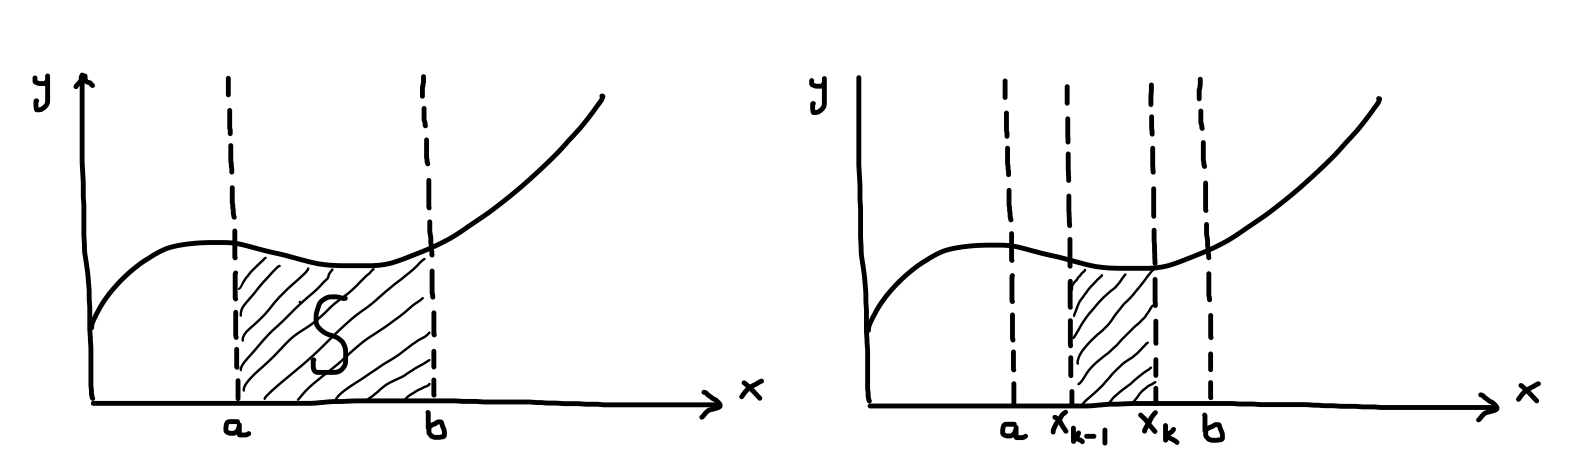
\includegraphics[width=14cm]{2_9_2_2}

\end{tabular}
\end{table} 

    
			\item $S=\int\limits_a^b|y(x)|\dx=\left|\begin{array}{c}
				x\in[a,\>b]\\y(x)<0
			\end{array} \right|\Rightarrow S=-\int\limits_a^bf(x)\dx,\>y=|y(x)|$ на $[a,\>b]$
			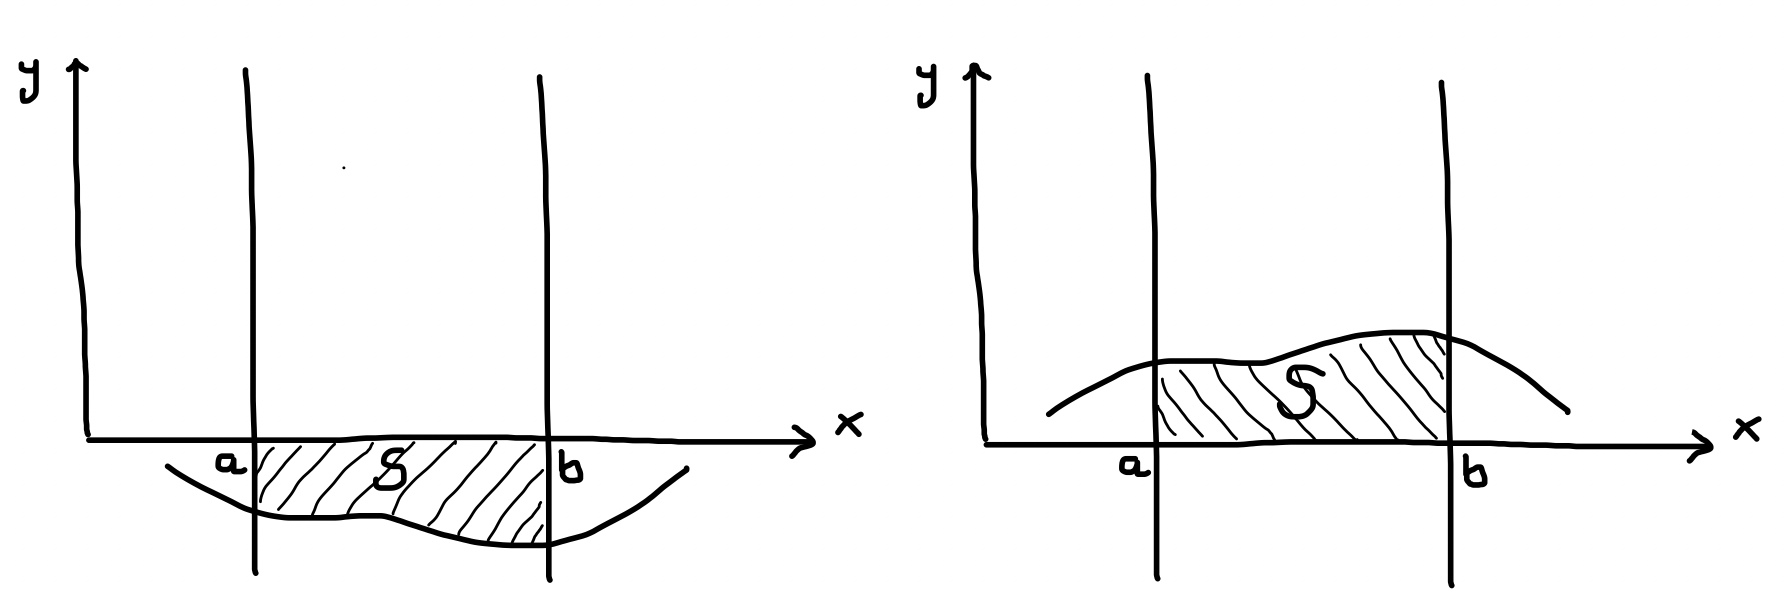
\includegraphics[width=14cm]{2_9_2_3}\newpage
			\item $S=\int\limits_a^b(y_2(x)-y_1(x))\dx$ \\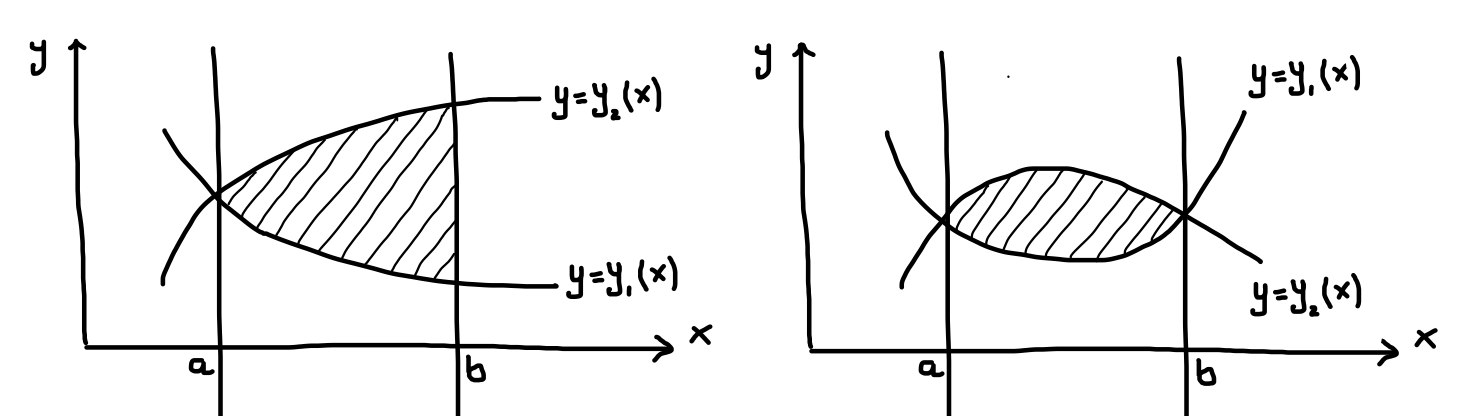
\includegraphics[width=14cm]{2_9_2_4}
			\item Криволинейная трапеция. \\$y=c,\>y=d,\>x=0,\>y=y(x),\>x=x(y),\>S=\int\limits_c^dx(y)\dy y$\\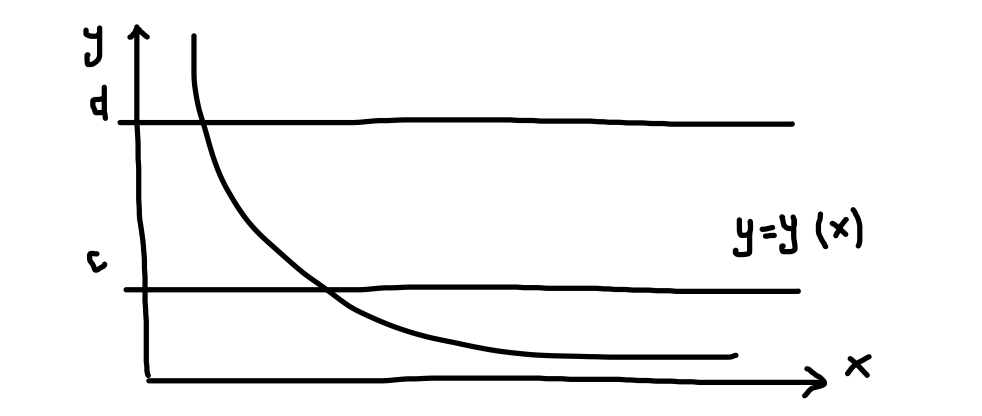
\includegraphics[width=14cm]{2_9_2_5}
		\end{enumerate}  
		\item Кривые заданы параметрическими уравнениями 
		\begin{enumerate}
			\item $L:\>\left\{\begin{array}{l}
				x=x(t)\\y=y(t)
			\end{array} \right.\>\alpha\leq t\leq\beta\begin{array}{l}
				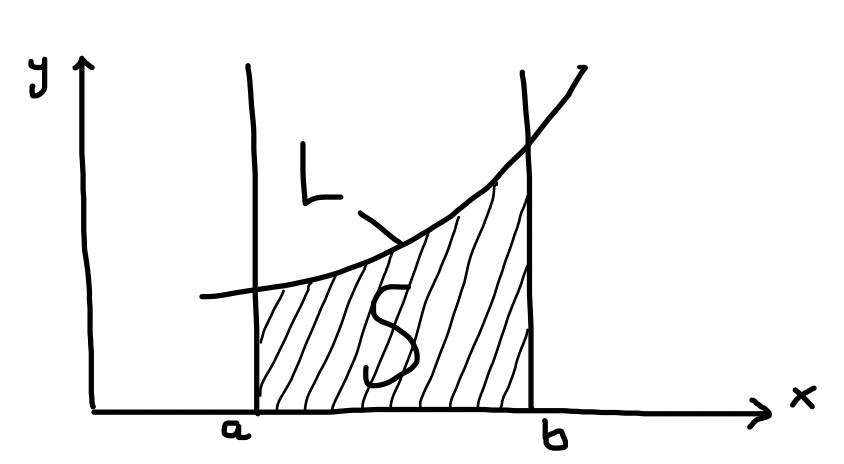
\includegraphics[width=4cm]{2_9_2_6}
			\end{array}\\$ Знаем: $S=\int_a^b y(x)\dx\\\left|\begin{array}{ll}
				y=y(t):&\dx=x'(t)\dy t\\
				x=x(t):&x=a,\>x(t)=a\to t=\alpha\\
				&x=b,\>x(t)=b\to t=\beta
			\end{array} \right|$ $$S=\int\limits_\alpha^\beta y(t)\>:\>x'(t)\dy t$$\newpage
			\item $S=\int\limits_c^dx(y)\dy y\\\left|\begin{array}{llll}
				y=y(t)&y=c:&y(t)=c\to t=\alpha&\\x=x(t)&y=d:&y(t)=d\to t=\beta&\dy y=y'(t)\dy t
			\end{array} \right|\begin{array}{c}
				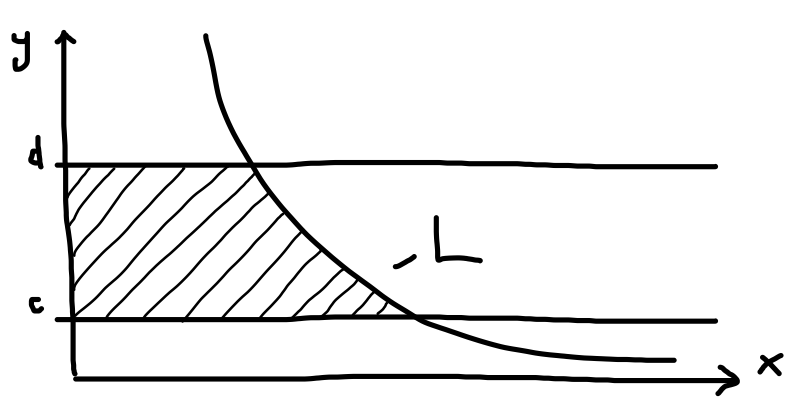
\includegraphics[width=4cm]{2_9_2_7}
			\end{array}$ $$S=\int\limits_\alpha^\beta x(t)\cdot y'(t)\dy t$$
		\end{enumerate}
		\begin{example}
			\begin{itemize}
				\item [1.] $S_\textrm{ф}$ - ограничена : $y_1=x^2-2x,\>y_2=Ox,\>x=3\\\begin{array}{c}
					 \\
					x\in[0,\>3]\\
					\tab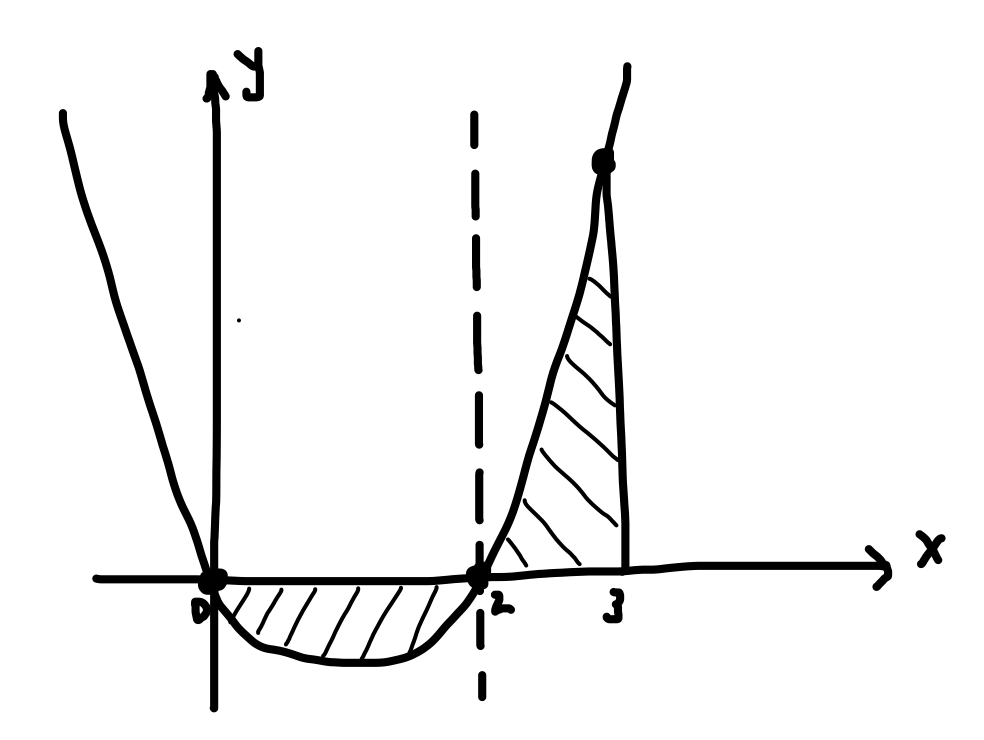
\includegraphics[width=4cm]{2_9_2_8}
				\end{array} \begin{array}{l}
					S=S_1+S_2\\S=-\int\limits_0^2(x^2-2x)\dx+\int\limits_2^3(x^2-2x)\dx=\dots=\\=\frac83
				\end{array}$
				\item [2.] $S_\textrm{эл},\>\frac{x^2}{a^2}+\frac{y^2}{b^2}=1\\\begin{array}{l}
					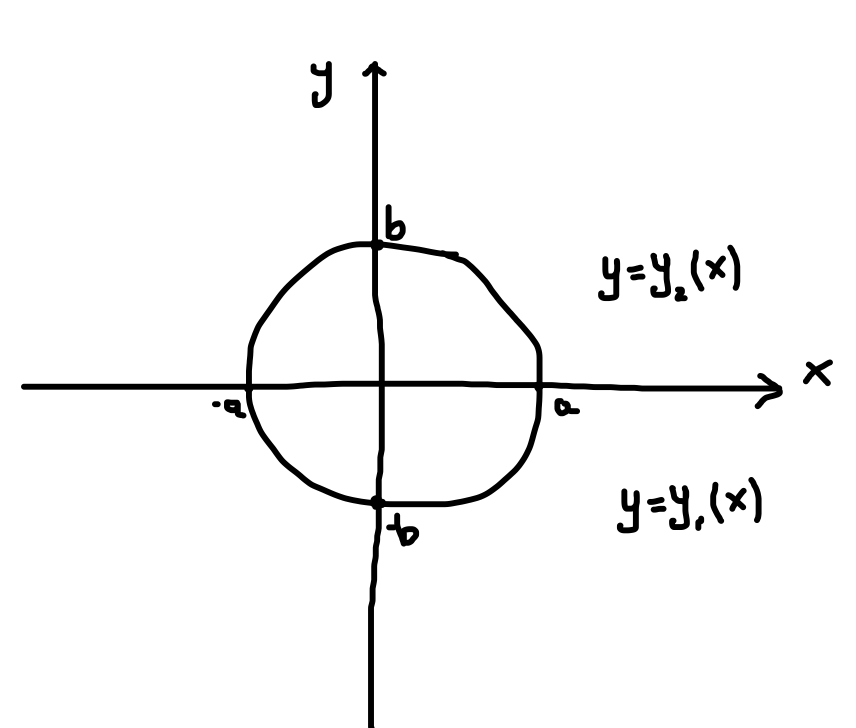
\includegraphics[width=4cm]{2_9_2_9}
				\end{array}\begin{array}{l}
					y_1=-b\sqrt{1-\frac{x^2}{a^2}}\\
					y_2=b\sqrt{1-\frac{x^2}{a^2}}\\
					S_\textrm{эл}=2\int\limits_{-a}^ab\sqrt{1-\frac{x^2}{a^2}}\dx=\left|\textrm{триг. замена} \right|
				\end{array}\\$ параметрическое уравнение эллипса \\$\left\{\begin{array}{l}
					x=a\cos t\\y=b\sin t 
				\end{array} \right.$ Симметрия $\Rightarrow S_\textrm{эл}=4S_1.\tab 0\leq t\leq 2\pi\\\begin{array}{l}
					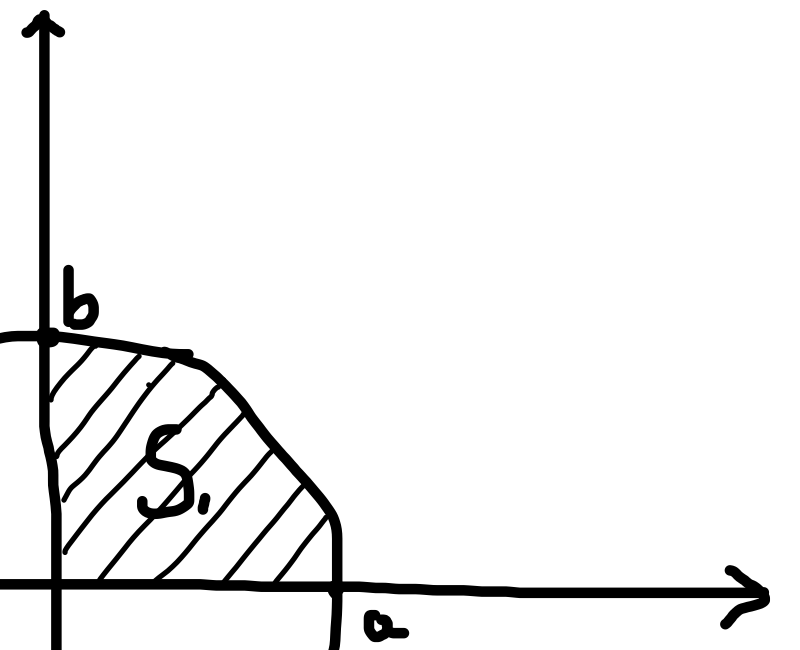
\includegraphics[width=2cm]{2_9_2_11}
				\end{array}\left\{\begin{array}{ll}
					x=a\cos t; & S_1=\int\limits_{\alpha}^\beta y(t)\cdot x'(t)\dy t=\\
					y=b\sin t; & =\int\limits_0^{\frac\pi2}(b\sin t-a\sin t)\dy t=
				\end{array} \right.\left|\begin{array}{c}
					x=0\\a\cos t=0;t=\frac{\pi}2\\x=a\\a\cos t=a;t=a
				\end{array} \right|\\=ab\int\limits_0^{\frac\pi2}\sin^2t\dy t=\frac{ab}2\int\limits_0^{\frac\pi2}(1-\cos^2t)\dy t=\frac{ab}2\left(t-\frac{\sin2t}2\right)\Big|_0^{\frac{\pi}2}=\frac{ab}2\left(\frac{\pi}2-0\right)=\\=\frac{\pi ab}4;\tab  S_\textrm{эл}=4S_1=\pi ab$
			\end{itemize}
		\end{example}\newpage
		
		\item Кривые, заданные в полярных координатах\\Площадь криволинейного сектора. Метод дифференциала:\\Пусть $S=S(\varphi)$ - площадь криволинейного сектора, причем $S(\alpha)=0,\>S(\beta)=S$ - некоторая площадь. Возьмем $\varphi\in(\alpha,\>\beta):\>\Delta S=S(\varphi+\Delta\varphi)-S(\varphi).\>\Delta S\approx\dy S.$ В качестве $\dy S$ возьмем площадь не криволинейного, а кругового сектора$\\(S_\textrm{сектора}=\frac{R^2\alpha}{2})\Rightarrow\dy S=\frac12\rho^2(\varphi)\dy\varphi.$ Интегрируем, получаем: $$S_\textrm{сектора}=\frac12\int\limits_\alpha^\beta\rho^2(\varphi)\dy\varphi $$
			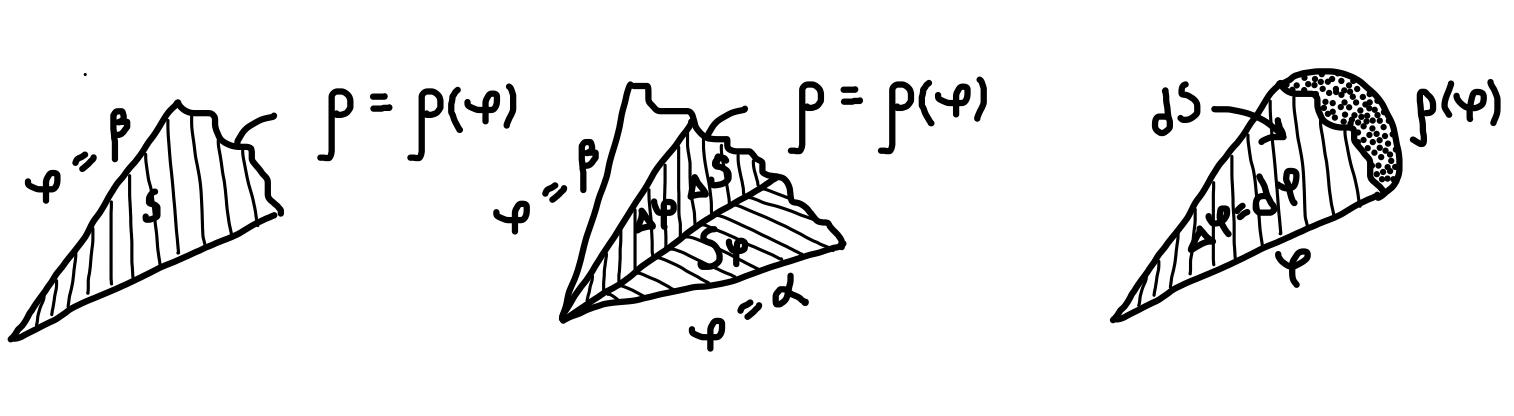
\includegraphics[width=14cm]{2_9_2_12}
			\begin{example}
				Найти $s_\phi:\>r=a\cos3\varphi\>(a>0)\\r>0\Rightarrow\cos3\varphi>0,\>-\frac\pi2+2\pi_n\leq 3\varphi \leq \frac\pi2+2\pi_n,\>-\frac\pi6+\frac{2\pi_n}3\leq\varphi\leq\frac\pi6+\frac{2\pi_n}3$ 
				\begin{enumerate} 
					\item $n=0:\tab -\frac\pi6\leq\varphi\frac\pi6\Rightarrow-\frac\pi2\leq3\varphi\leq\frac\pi2,$
					\item $n=1:\tab \frac\pi2\leq\varphi\leq\frac{5\pi}6\Rightarrow\frac{3\pi}2\leq3\varphi\leq\frac{5\pi}2,$
					\item $n=2:\tab \frac{7\pi}6\leq\varphi\leq\frac{3\pi}2\Rightarrow\frac{7\pi}2\leq3\phi\leq\frac{9\pi}2$ \begin{itemize}
							\item [1)] $3\varphi=-\frac\pi2\Rightarrow\varphi=-\frac\pi6\Rightarrow\cos3\varphi=0\Rightarrow r=0\\3\varphi=0\Rightarrow\varphi=0\Rightarrow\cos3\varphi=1\Rightarrow r=a\\3\varphi=\frac\pi2\Rightarrow\varphi=\frac\pi6\Rightarrow\cos3\varphi=0\Rightarrow r=0\\$ \item[2)], 3) - рассуждения аналогичны
					\end{itemize}
				\end{enumerate} $S=6S_1,\>S_1=\frac12\int\limits_0^\frac\pi6r^2(\varphi)\dy \varphi=\frac{a^2}2\int\limits_0^\frac\pi6\cos^23\varphi\dy\varphi=\frac{a^2}4\int\limits_0^\frac\pi6(1-\cos6\varphi)\dy\varphi=\\=\frac{a^2}4(\varphi+\frac16\sin6\varphi)\Big|_0^{\frac{\pi}6}=\frac{a^2}4\cdot\frac\pi6\Rightarrow S_\phi=\frac{6a^2\pi}{4\cdot 6}=\frac{a^2\pi}4$
				\begin{center}
					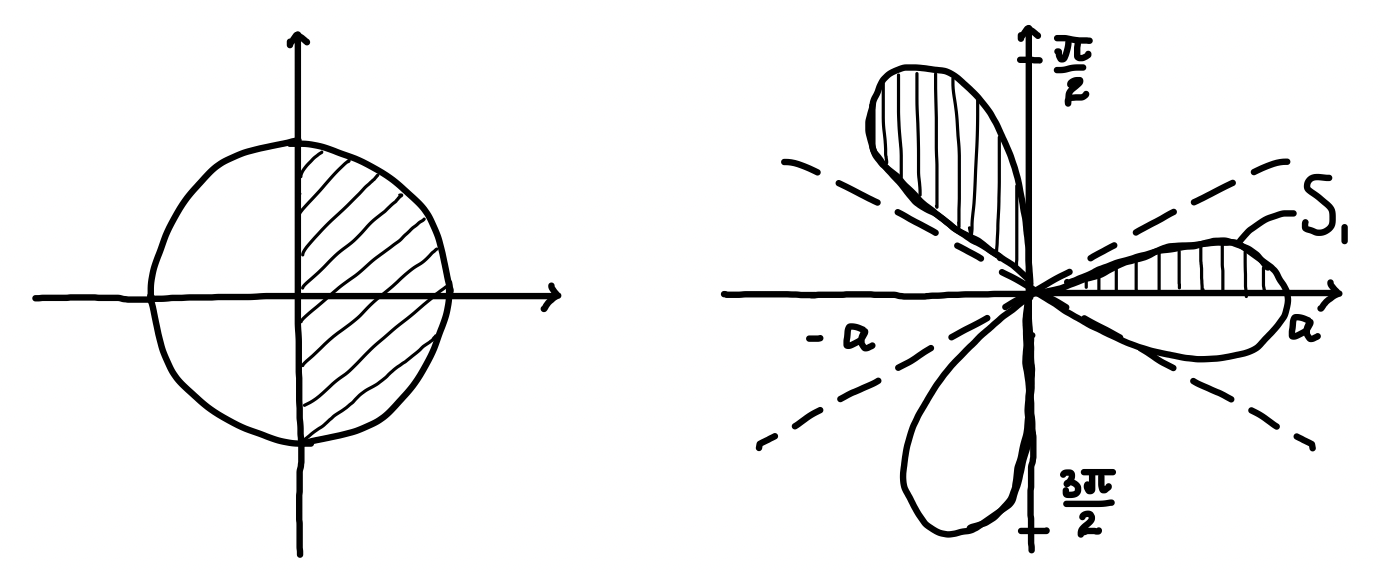
\includegraphics[width=9cm]{2_9_2_13}
				\end{center}
			\end{example}
\end{enumerate}
\subsection{Вычисление длин дуг кривых}
\begin{enumerate}
	\item Кривая заданная явно: $y=y(x)\\\begin{array}{l}
		\textrm{Под длинной кривой }AB\textrm{ понимаю предел,}\\\textrm{к которому стремится длинна ломаной, вписанной}\\\textrm{в эту кривую, когда длина максимального звена}\\\textrm{стремится к нулю.} AB:\>y=y(x),\>x\in[a,\>b]\\\textrm{Пусть } L\textrm{ - длина } AB.\textrm{ Введем функцию } f(x):\\l(x)\textrm{ - длина }AM.\>(M(x,\>y(x)),\>a\leq x\leq b),\\\textrm{ при этом: }l(a)=0,\>l(b)=L\textrm{ - искомая. }\Delta l\textrm{ - дуга}\\MN,\>\dy l(x)\overset{\textrm{def}}{\underset{\dy f}{\longeq}}l'(x)\dx,\>l'(x)\overset{\textrm{def f'}}{{\longeq}}\lim\limits_{\Delta x\to0}\frac{\Delta l}{\Delta x}=\
	\end{array} \begin{array}{c}
		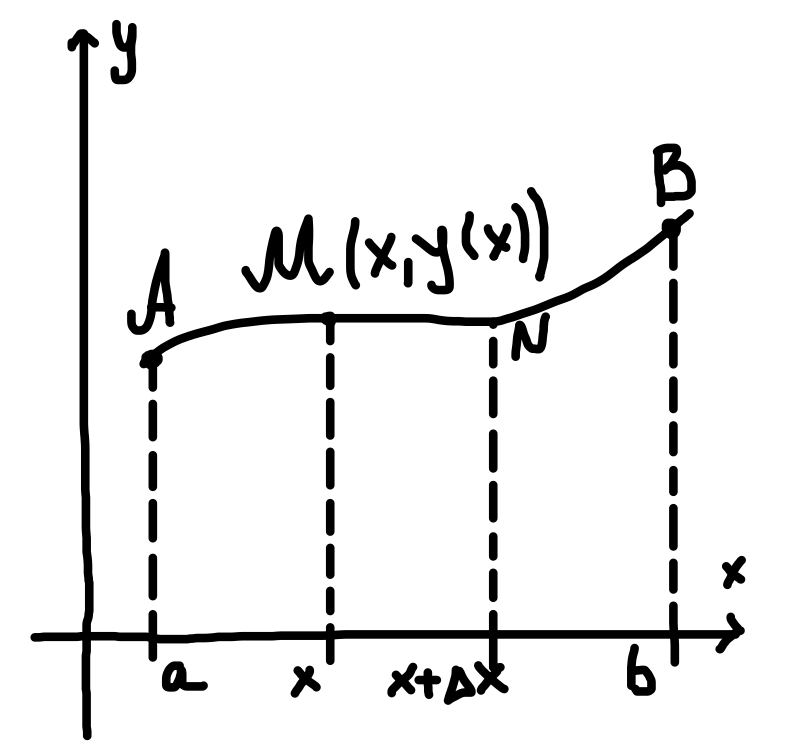
\includegraphics[width=5cm]{2_9_2_14}
	\end{array}\\=\lim\limits_{\Delta x\to0}-\frac{\sqrt{(\Delta x)^2+(\Delta y)^2}}{\Delta x}=\lim\limits_{\Delta x\to0}\sqrt{1+\left(\frac{\Delta x}{\Delta y} \right)^2}=\sqrt{1+(y'(x))^2},\>\dy l=\sqrt{1+(y'(x))^2}\dx$ $$L=\int\limits_a^b\dy l, \textrm{ т.е. }L=\int\limits_a^b\sqrt{1+(y'(x))^2}\dx$$
	\begin{remark}
		$\\\begin{array}{c}
			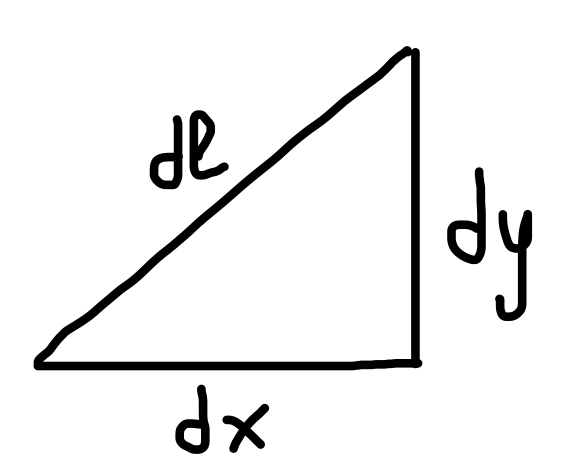
\includegraphics[width=3cm]{2_9_2_15}
		\end{array}\begin{array}{l}
			\textrm{Величина  } \dy l \textrm{называется дифференциалом длины дуги.}\\\dy l=\sqrt{(\dx)^2+(\dy y)^2},\>\dy y=y'(x)\dx
		\end{array}$
	\end{remark}
	\item Дина дуги кривой, заданной параметрически.\\$L=\left\{\begin{array}{l}
		x=x(t),\\y=y(t)
	\end{array}\right.\alpha\leq t\leq\beta\\L=\int\dy l=\left|\begin{array}{ll}
		\dx=x'(T)\dy t, & \dy l=\sqrt{1+(y'(x)^2}\dx = \sqrt{1+\left(\frac{y_t'}{x_t'}\cdot x_t'\dy t \right)}=\\
		\dy =y'(t)\dy t, & =\sqrt{(x_t')^2+(y_t')^2}\dy t
	\end{array} \right|\textcircled{=}$
	\begin{remark}
		Т.к. величина $\dy l>0,\>\sqrt{\dots}>0\Rightarrow\dy t>0.$ Это означает, что по $t$ при вычислении длин кривой пределы всегда расставляються от меньшего к большему
	\end{remark}
	$$\textcircled{=}\>L=\int\limits_a^b\sqrt{(x_t')^2+(y_t')^2}\dy t$$
	\begin{example}
		Найти длину окружности: $x^2+y^2=R^2.$ Параметрическое уравнение окружности: 
		$\left\{\begin{array}{l}
			x=R\cos t,\\y=R\sin t,
		\end{array}\right. t\in[0,\>2\pi]\\x_t'=-R\sin t,\>(x_t')^2+(y_t')^2=(-R\sin t)^2+(R\cos t)^2=R^2,\>y_t'=R\cos t\\l_I=\int\limits_0^{\frac{\pi}2}\sqrt{(x_t')^2+(y_t')^2}\dy t=R\int\limits_0^{\frac\pi2}\dy t=\frac{R\pi}2\Rightarrow l=4l_I=2\pi R$
	\end{example}
	\item Кривая, заданная уравнением в полярных координатах
		$\\\begin{array}{l}
			r=r(\varphi),\>\alpha\leq\varphi\leq\beta\\
			\dy l=\sqrt{(\dx)^2+(\dy y)^2}
		\end{array}\tab\left\{\begin{array}{l}
			x=r(\varphi)\cos\varphi\\
			y=r(\varphi)\sin\varphi
		\end{array} \right.\\x_\varphi'=r'(\varphi)\cos\varphi+r(\varphi)\cdot(-\sin\varphi)\\(x_\varphi')^2=(r'(\varphi))^2\cos^2\varphi-2r(\varphi)\cdot r(\varphi)\cos\varphi\sin\varphi-r^2(\varphi)\sin^2\varphi,\\y_\varphi'=r'(\varphi)\sin\varphi+r(\varphi)\cos\varphi\\(y_\varphi')^2=(r'(\varphi))^2\sin^2\varphi+2r(\varphi)\cdot r'(\varphi)\cdot\cos\varphi\sin\varphi+r^2(\varphi)\cos^2\varphi,\\(x_\varphi')^2+(y_\varphi')^2=(r'(\varphi))^2+r^2(\varphi).$ $$l=\int\limits_\alpha^\beta\sqrt{(x_\varphi')^2+(y_\varphi')^2\dy\varphi}=\int\limits\limits_\alpha^\beta\sqrt{(r'(\varphi))^2+r^2(\varphi)}\dy\varphi$$
		\begin{example}
			Найти длину кривой $r=a(1+\cos\varphi)\\\tab\begin{array}{l}
				\varphi=0\Rightarrow\cos\varphi=1\Rightarrow r=2a\\
				\varphi=\frac\pi2\Rightarrow\cos\varphi=0\rightarrow r=a\\
				\varphi=\pi\Rightarrow\cos\varphi=-1\Rightarrow r=0\\
				
			\end{array} \begin{array}{c}
				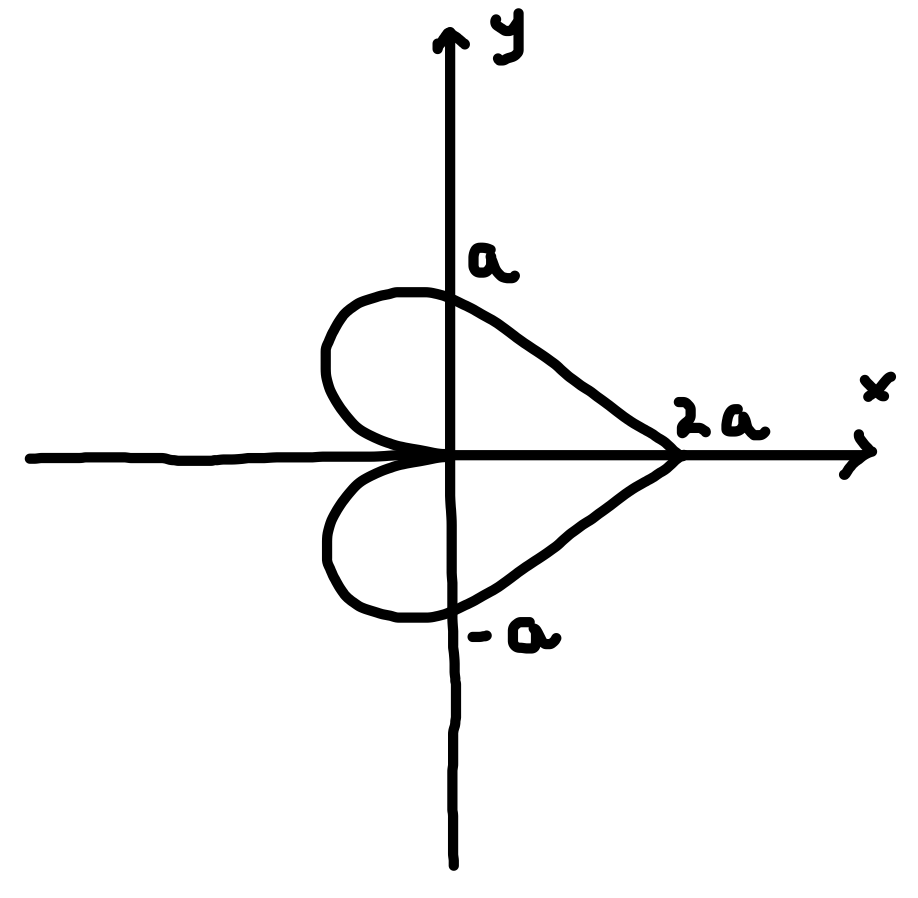
\includegraphics[width=3cm]{2_9_2_16}
			\end{array}\\\frac12l=\int\limits_0^\pi\sqrt{(r')^2+r^2}\dy\varphi,\\(r_\varphi')=a(-\sin\varphi),\>(r')^2=a^2\sin^2\varphi,\>r^2=a^2(1+2\cos\varphi+\cos^2\varphi)\\\frac12l=\int\limits_0^\pi\sqrt{a^2(\sin^2\varphi+1+2\cos\varphi+\cos^2\varphi)}\dy\varphi=a\int\limits_0^\pi\sqrt{2(1+\cos\varphi)}\dy\varphi=\\=a\int\limits_0^\pi\sqrt{4\cos^2\frac\varphi2}\dy\varphi=2a\int\limits_0^\pi\left|\cos\frac\varphi2\right|\dy\varphi=\left|\begin{array}{c}
				\varphi\in[0,\>\pi]\\\cos\frac\varphi2>0
			\end{array} \right|=2a\int\limits_0^\pi\cos\frac\varphi2\dy\varphi=\\=2a\sin\frac\varphi2\cdot2\Big|_0^\frac\pi2=4a(\sin\frac\pi2-\sin0)=4a,\>l=2\cdot4a=8a$  
		\end{example}
\end{enumerate}
\subsection{Вычисление объемов тел}
\begin{enumerate} 
	\item Объем тела по известным поперечным сечением (нарезаная колбаса??)$\\\begin{array}{c}
		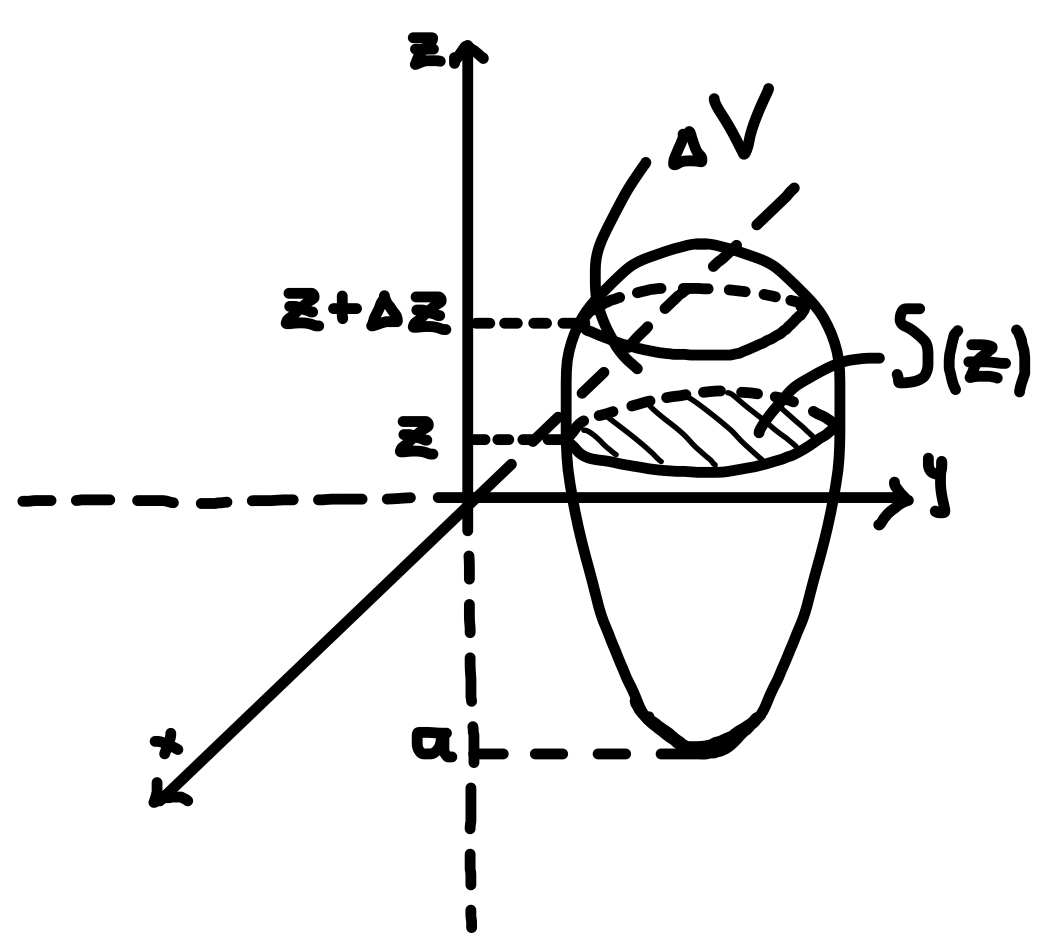
\includegraphics[width=8cm]{2_9_2_17}
	\end{array}\begin{array}{l}
		\forall \zstroke\in[a,\>b]\textrm{ известна площадь} S(\zstroke)\\\textrm{сечение этого тела плоскостью,}\\\textrm{перпендикулярной оси } O\zstroke.\\\textrm{Пусть } V(\zstroke)\textrm{ - объем тела,}\\\textrm{ограниченный }s(\zstroke)\textrm{ и } a\textrm{ (от нижней}\\\textrm{части до }S(\zstroke)). \dy V=|h=\dy\zstroke|=\\=S(\zstroke)\dy\zstroke\Rightarrow V=\bigintsss\limits_a^bS(\zstroke)\dy\zstroke
	\end{array}$
	\begin{example}
		Найти объем тела: $\frac{x^2}{a^2}+\frac{y^2}{b^2}+\frac{\zstroke^2}{c^2}=1\\$ При фиксированном $\zstroke\tab(-c\leq\zstroke\leq c):\\\begin{array}{c}
			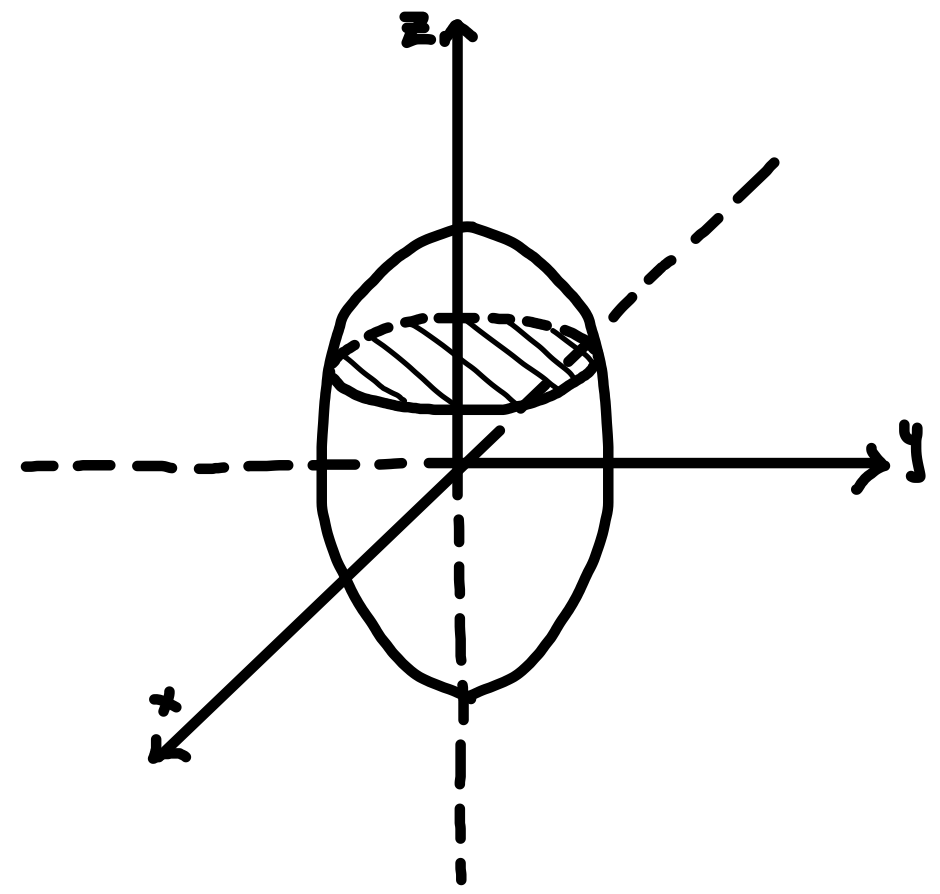
\includegraphics[width=5cm]{2_9_2_18}
		\end{array}\begin{array}{l}
			\frac{x^2}{a^2}+\frac{y^2}{b^2}+\frac{\zstroke^2}{c^2}=1,\>\frac{x^2}{a^2}+\frac{y^2}{b^2}=1-\frac{\zstroke^2}{c^2},\>\frac{x^2}{a^2}+\frac{y^2}{b^2}=\frac{c^2-\zstroke^2}{c^2}\\\frac{x^2}{a^2\cdot\frac{c^2-\zstroke^2}{c^2}}+\frac{y^2}{b^2\cdot\frac{c^2-\zstroke^2}{c^2}}=1,\>\frac{x^2}{\left(\frac ac\cdot\sqrt{c^2-\zstroke^2}\right)^2}+\frac{y^2}{\left(\frac bc\cdot\sqrt{c^2-\zstroke^2}\right)^2}=1\\\textrm{ - уравнение эллипса с полуосями: }\\a_1=\frac ac\cdot\sqrt{c^2-\zstroke^2},\>b_1=\frac bc\cdot\sqrt{c^2-\zstroke^2}.\\\textrm{ Известно: }S(\zstroke)\textrm{ - площадь эллипса} = \pi a_1b_1=\\=\pi\frac{ab}c(c^2-\zstroke^2).\\V=\int\limits_{-c}^c\pi\frac{ab}c(c^2-\zstroke^2)\dy\zstroke=\frac{\pi ab}{c^2}\left(c^2\zstroke-\frac {\zstroke^3}3\right)\bigg|_{-c}^c=\\=\frac{\pi ab}{c^2}\left(c^3+c^3-\frac{c^3}3-\frac{c^3}3\right)=\frac43\pi abc
		\end{array}$ 
	\end{example}\newpage
	\item Объем тела вращения 
		\begin{enumerate} 
			\item Вращение воукруг оси $Ox$\\ $\begin{array}{c}
				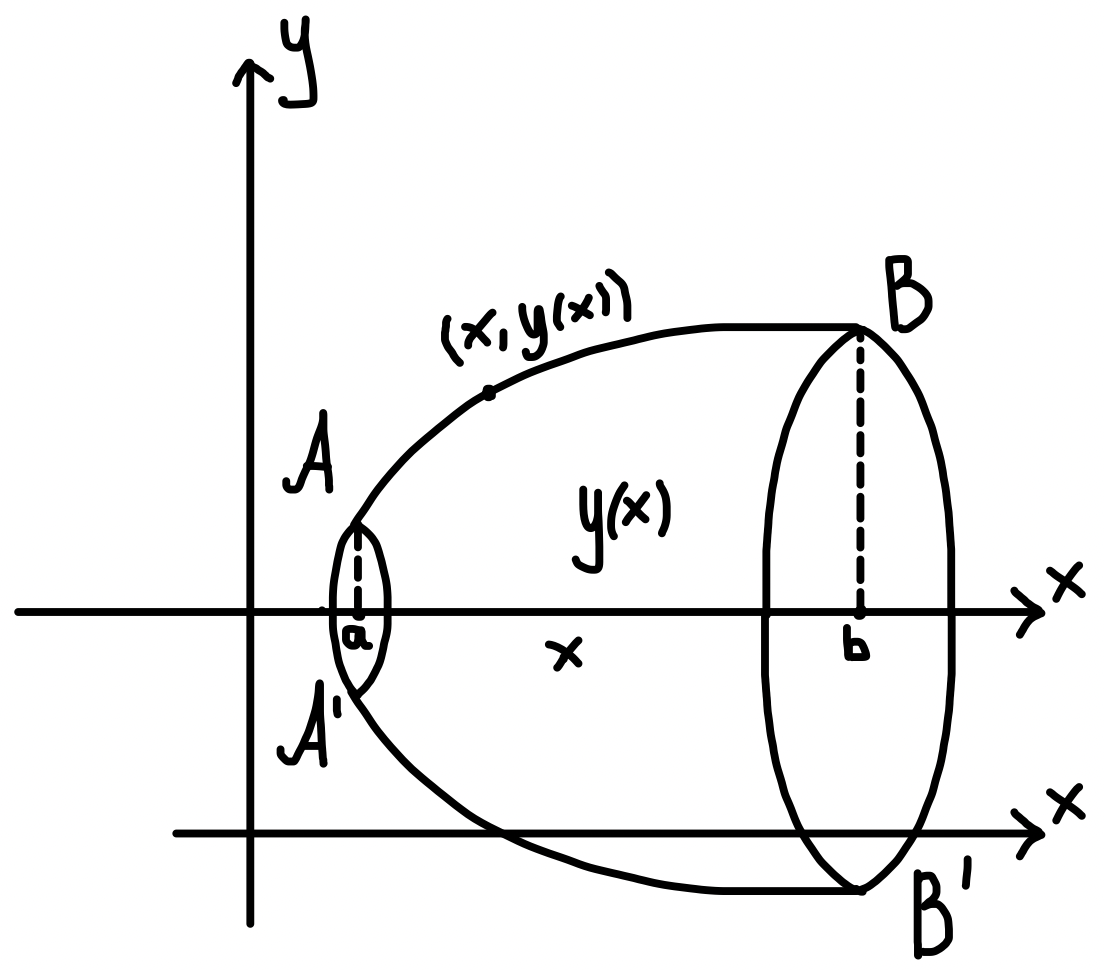
\includegraphics[width=8cm]{2_9_2_19}
			\end{array}\begin{array}{l}
				AB:\>y=y(x),\>a\leq x\leq b\\S(x)=\pi y^2(x)\>(S\textrm{ кргуа})\\\\V=\pi\bigintsss\limits_a^by^2(x)\dx
			\end{array}$ \begin{remark}
				$\\\begin{array}{c}
					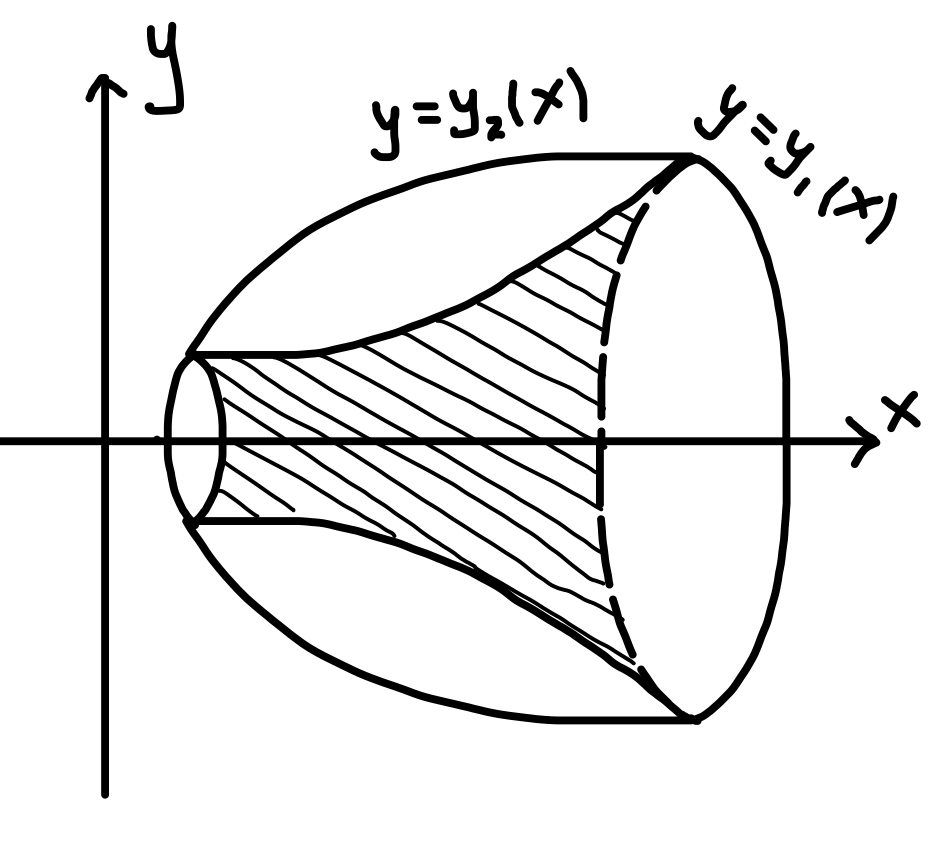
\includegraphics[width=5cm]{2_9_2_20}
				\end{array}V=V_1-V_2=\pi\bigintsss\limits_a^b\left(y_2^2(x)-y_1^2(x)\right)\dx$
			\end{remark}
		\end{enumerate}
\end{enumerate}


























\end{document}
